\documentclass [a4paper,normaltoc,normalfigtabnum, header, espacoumemeio, capchap, capsec, cappre, 12pt,notimes]{abntpoli}

\usepackage{xcolor}
\usepackage{graphicx}
\usepackage{acronym}
\usepackage[brazil]{babel}
\usepackage[T1]{fontenc}
\usepackage{amsmath}
\usepackage{amssymb}
\usepackage{listings}
\usepackage{tocbibind}
\usepackage[labelsep=endash, font=footnotesize]{caption}
\usepackage[alf, abnt-emphasize=bf]{abntcitepoli}
\usepackage[final]{listofsymbols}
\usepackage{url}
\usepackage{textcomp}
\usepackage{imakeidx}
\usepackage{subfig}
\usepackage[section]{placeins}
\usepackage{etoolbox}
\usepackage{dsfont} % fontes matem�ticas duplas como N, Z, R, para designar conjuntos
\usepackage[subfigure]{tocloft}
\usepackage[final]{pdfpages}
% Adicionadas por mim
\usepackage{tabu}
\usepackage{enumitem}
\usepackage{pgfgantt}
\usepackage[latin1]{inputenc}
\DeclareRobustCommand{\VAN}[3]{#2} % set up for citation of dutch names
\DeclareRobustCommand{\DE}[3]{#2}
\usepackage{multirow}
\setcounter{secnumdepth}{5}

\usepackage{array}
\newcolumntype{L}[1]{>{\raggedright\let\newline\\\arraybackslash\hspace{0pt}}m{#1}}
\newcolumntype{C}[1]{>{\centering\let\newline\\\arraybackslash\hspace{0pt}}m{#1}}
\newcolumntype{R}[1]{>{\raggedleft\let\newline\\\arraybackslash\hspace{0pt}}m{#1}}

\renewcommand{\familydefault}{\sfdefault}

\makeindex[title=�ndice]


% 

\setcounter{lofdepth}{1}


\newlength\tablelen
\settowidth\tablelen{\tablename\;}
\addtolength\cfttabnumwidth{\tablelen}
\renewcommand\cfttabpresnum{\tablename\;}
\renewcommand\cfttabaftersnum{\,--\;}

\newlength\figlen
\settowidth\figlen{\figurename\;}
\addtolength\cftfignumwidth{\figlen}
\renewcommand\cftfigpresnum{\figurename\;}
\renewcommand\cftfigaftersnum{\,--\;}


\graphicspath{{./figuras/}}

\allowdisplaybreaks


   
   %\lhead{\thechapter}
   
   

\begin{document}
	\pagenumbering{roman}
	
	
\autor{Pablo Alejandro de Abreu Urbizag�stegui}
\titulo{BLANK}
\orientador{Andr� Fabio Kohn}
\local{S�o Paulo}
\areadeconcentracao{Sistemas Eletr�nicos}
 \comentario{Disserta��o apresentada � Escola Polit�cnica da \mbox{Universidade} de S�o Paulo para a obten��o do t�tulo de Mestre em Ci�ncias}
\data{2018}
\capa
\folhaderosto





    \includepdf{EPUSP-Catalogacao-na-Fonte.pdf}

    %%%%%%%%%%%%%%% Folha de aprova��o
    \begin{folhadeaprovacao}
        \noindent Urbizagastegui, Pablo Alejandro de Abreu.
        \textbf{Modelagem de c�lulas de Renshaw e sua utiliza��o
        em simula��es do sistema neuromuscular}.
        2019. 98 f. Disserta��o (Mestrado) - Escola Polit�cnica,
        Universidade de S�o Paulo, S�o Paulo, 2019. \\
        \\
        
        \noindent Aprovado em:
        \begin{center}
            Banca Examinadora
        \end{center}

        \noindent Prof. Dr. \hspace{0.7cm}\rule{0.7\textwidth}{.4pt} \\
        \noindent Institui��o: \hspace{0.4cm}\rule{0.7\textwidth}{.4pt} \\
        \noindent Julgamento: \hspace{0.2cm}\rule{0.7\textwidth}{.4pt} \\
        \\
        \noindent Prof. Dr. \hspace{0.7cm}\rule{0.7\textwidth}{.4pt} \\
        \noindent Institui��o: \hspace{0.4cm}\rule{0.7\textwidth}{.4pt} \\
        \noindent Julgamento: \hspace{0.2cm}\rule{0.7\textwidth}{.4pt} \\
        \\
        \noindent Prof. Dr. \hspace{0.7cm}\rule{0.7\textwidth}{.4pt} \\
        \noindent Institui��o: \hspace{0.4cm}\rule{0.7\textwidth}{.4pt} \\
        \noindent Julgamento: \hspace{0.2cm}\rule{0.7\textwidth}{.4pt} \\
        \\
    \end{folhadeaprovacao}
    %%%%%%%%%%%%%%%%%%%%%%%%%%%%%%%%%%%

	\pretextualchapter{Agradecimentos}

Primeiramente, agrade�o ao Prof. ....

Aos colegas ...

Aos meus pais ....

....

Por fim, � quem me financiou.
	
	\newpage
	\begin{resumo}
\noindent Urbizagastegui, Pablo Alejandro de Abreu.
\textbf{Modelagem de c�lulas de Renshaw e sua utiliza��o
em simula��es do sistema neuromuscular}.
2019. 98 f. Disserta��o (Mestrado) - Escola Polit�cnica,
Universidade de S�o Paulo, S�o Paulo, 2019. \\
\\
%As C�lulas de Renshaw s�o interneur�nios inibit�rios localizados na
%medula espinhal se mam�feros como gatos, ratos e seres humanos. Por
%desempenharem um papel central no circuito de inibi��o recorrente,
%acredita-se que as c�lulas de Renshaw sejam importantes para a gera��o
%e coordena��o de atividades musculares. Entretanto, at� hoje n�o se sabe
%qual a fun��o principal desse neur�nio.
O objetivo principal
desse trabalho foi realizar um estudo computacional sobre as influ�ncias
da c�lula de Renshaw sobre motoneur�nios em diferentes situa��es, mas
tamb�m envolveu parametriza��es e recomenda��es de t�cnicas para melhorar
o desempenho do sistema de simula��o utilizado.
O ajuste de par�metros e as simula��es foram guiados por
dados experimentais de gatos dispon�veis na literatura.
Os resultados obtidos, al�m de mostrar que o modelo utilizado
foi capaz de reproduzir de forma satisfat�ria v�rias observa��es experimentais,
sugerem que as c�lulas de Renshaw podem afetar a for�a muscular gerada
e a taxa de disparos e o recrutamento de motoneur�nios.
Dentre as simula��es e an�lises realizadas, destacam-se os fatos de que,
quando as c�lulas de Renshaw estava presentes, houve maior tend�ncia a
ocorrer invers�es na ordem de recrutamento, maior velocidade no
desenvolvimento da for�a muscular e a capacidade de diminuir oscila��es
em 10 Hz por meio de cancelamento de fases.
O modelo foi disponibilizado como uma ferramenta \textit{open source},
facilitando a reproduzibilidade e extens�o dos assuntos abordados.

\noindent Palavras-chave: C�lula de Renshaw. Neur�nios motores.
Neurofisiologia. Simula��o.
\end{resumo}

\begin{abstract}

\noindent Urbizagastegui, Pablo Alejandro de Abreu.
\textbf{Modelling of Renshaw cells and its utilization in simulations of the
neuromuscular system}.
2019. 98 f. Disserta��o (Mestrado) - Escola Polit�cnica,
Universidade de S�o Paulo, S�o Paulo, 2019. \\
\\
The present work carries out a computational study on
the influences of Renshaw cell on motoneurons in different situations,
but also involves parametrization and recommendations of techniques
to improve the performance of the simulation system utilized. The
adjustments of parameters and simulations were guided by cat experimental
data available in the literature. The results obtained not only showed
that the model used could properly reproduce several experimental
observations, but also suggested that Renshaw cells can affect muscle
strength and motoneuronal rate and recruitment. Among the simulations
and analyzes performed, it should be emphasized that when the Renshaw
cells were included there was a greater tendency for inversions in the
orderly recruitment of motoneurons to occur, greater speed of muscle force
development and decrease of oscillations at 10 Hz by phase cancellation.
The model was distributed as an open source tool, facilitating the
reproducibility and extension of the observations described.

\noindent Keywords: Renshaw cell. Motoneurons. Neurophysiology. Simulation.
\end{abstract}

	
%	\renewcommand\listfigurename{Lista de Figuras}
	
	\listadefiguras
	\listadetabelas
	%%% modifica a maneira de apresentar a lista de siglas
	\def\bflabel#1{{{\textsf{#1}}\hfill}}
	\renewenvironment{AC@deflist}[1]%
	      {\if AC@nolist%
		\else%
		    \raggedright\begin{list}{}%
		    {\settowidth{\labelwidth}{\textsf{#1}+8pt}%
		    \setlength{\leftmargin}{\labelwidth}%
		    \setlength{\itemsep}{0.5pt}%
		    \addtolength{\leftmargin}{\labelsep}%
		    \renewcommand{\makelabel}{\bflabel}}%
		 \fi}%
		{\if AC@nolist%
		  \else%
		    \end{list}%
		\fi}%

\pretextualchapter{Lista de Siglas}

\begin{acronym}[NARMAX]
    \acro{ACh}[ACh]{Acetilcolina}
    \acro{AHP}[AHP]{Hiperpolariza��o p�s-potencial de a��o (do ingl�s \textit{Afterhyperpolarization})}
    \acro{CR}[CR]{C�lula de Renshaw}
    \acro{CST}[CST]{Trem de disparos cumulativo (do ingl�s \textit{Cumulative Spike Train})}
    \acro{CVM}[CVM]{Contra��o volunt�ria m�xima}
    \acro{EMG}[EMG]{Eletromiografia}
    \acro{FxI}[FxI]{Frequ�ncia de disparo \textit{versus} corrente injetada}
    \acro{FF}[FF]{Unidade motora de contra��o r�pida e fadiga r�pida (do ingl�s \textit{fast fatiguing})}
    \acro{FR}[FR]{Unidade motora de contra��o r�pida e resistente � fadiga (do ingl�s \textit{fast fatigue resistant})}
    \acro{IN}[IN]{Interneur�nio}
    \acro{MN}[MN]{Motoneur�nio}
    \acro{PEPS}[PEPS]{Potencial excitat�rio p�s-sin�ptico}
    \acro{PIPS}[PIPS]{Potencial inibit�rio p�s-sin�ptico}
    \acro{S}[S]{Unidade motora de contra��o lenta (do ingl�s \textit{slow})}
    \acro{SNC}[SNC]{Sistema nervoso central}
\end{acronym}

	\renewcommand\symheadingname{Lista de S�mbolos}
\renewcommand\symheading{\pretextualchapter{Lista de S�mbolos}}

\opensymdef
	\newsym[S�mbolo 1]{A}{\alpha}
	\newsym[S�mbolo 2]{X}{x}	
\closesymdef


	\listofsymbols	
	%\lhead{\thechapter}
	
	\sumario	
	
	%\pagestyle{fancyplain}
	\chapter{Introdu��o}
\label{cap:intro}

O objetivo desse trabalho � estudar as C�lulas de Renshaw e suas fun��es 
usando modelos computacionais realistas. A maioria dos dados usados aqui v�m
de experimentos realizados em membros inferiores de gatos. Como esse tipo de
experimento raramente � realizado hoje em dia, esses dados atualmente s�o
obtidos de ratos. Dessa forma, dados de ratos ser�o usados com cautela, com 
o devido aviso.
%The goal of the present work is to study the Renshaw cells and its functions
%using realistic computational models. Most of the data used here comes from
%experiments carried out on the cat hindlimb. As cat experiments are seldom
%performed nowadays, most of the recent data on the Renshaw cells come from 
%rat. Therefore, rat data will be used with caution and expressly indicated.

\section{O Sistema Motor}
O \textbf{Sistema Nervoso Central} � composto pelo c�rebro e pela 
\textbf{coluna espinhal}. O segundo � subdividido em cervical, tor�cico,
lombar e sacral, sendo cada um desses divididos em v�rios segmentos. A
coluna espinhal recebe e processa informa��o de m�sculos, articula��es e pele
e controla movimentos. Nesse contexto, o termo \textbf{aferente} � usado para
identificar sinais chegando � coluna espinhal, enquanto sinais entregues aos
m�sculos s�o chamados de \textbf{eferentes} \cite{kandel13}.
%The \textbf{central nervous system} (CNS) comprises the brain and the
%\textbf{spinal cord} (SC).
%The latter is further subdivided into cervical, thoracic, lumbar, and sacral,
%where each of these regions contains several segments.
%The SC receives and processes information from muscles, joints, and skin and 
%controls movement. In this context, the term \textbf{afferent} is used to
%identify
%the signals reaching the SC, whereas signals delivered to muscles are named
%\textbf{efferent} \cite{kandel13}.


O tipo de m�sculo estudado aqui � o \textbf{m�sculo esquel�tico}, que �
respons�vel por movimentar os ossos, olhos, inala��o e exala��o, controlar
express�es faciais e fala \cite{bear16}. Movimentos que diminuem o �ngulo
entre um segmento e seu segmento proximal s�o chamados de flex�o,
enquanto movimentos que aumentam esse �ngulo s�o chamados de
extens�o \cite{oxford}. Sendo assim, m�sculos podem ser
classificados como \textbf{flexores} e \textbf{extensores}. Se eles t�m a 
mesma fun��o, s�o chamados de \textbf{sinergistas} um do outro. Por outro
lado, se puxam a articula��o para lados opostos, s�o chamados de
\textbf{antagonistas} \cite{bear16}.
%The type of muscle studied herein is the \textbf{skeletal muscle}, which
%functions to move bones around joints, eyes within the head,
%inhalation/exhalation, control facial expression, and speech \cite{bear16}.
%Movements that decrease the angle between a segment and its proximal segment are
%described as flexion, whereas movements that increase it are called extension
%\cite{oxford}. Therefore, muscles can be classified as 
%\textbf{flexors} and \textbf{extensors}. If muscles work together, they are
%called
%\textbf{synergists} of one another. If they pull a joint on the opposite
%direction, they are called \textbf{antagonists} to one another \cite{bear16}.

Em cada m�sculo esquel�tico existem centenas de fibras musculares. Elas s�o
importantes n�o somente para a gera��o de for�a, mas tamb�m para
\textbf{propriocep��o}, j� que o \textbf{fuso muscular}, que consiste em
v�rias fibras esquel�ticas especializadas contidas em umas c�psula fibrosa,
fornece informa��o sobre o comprimento do m�sculo.
%Within each skeletal muscle there are hundreds of muscle fibers. They are
%important not only for force generation, but also for \textbf{proprioception},
%since the \textbf{muscle spindle}, which consists of several types of specialzed
%skeletal muscle fibers contained in a fibrous capsule, provides feedback about
%muscle length.

\section{A Circuitaria da Coluna Espinhal}
Um corte transversal da coluna espinhal � mostrado na Figura \ref{fig:ce}. O
n�cleo central � a \textbf{mat�ria cinzenta}, que cont�m o corpo de c�lulas
nervosas. A \textbf{subst�ncia branca} em volta dessa regi�o � abriga ax�nios
ascendentes e descendentes. A subst�ncia cinza ainda � subdividida em
\textbf{corno ventral} e \textbf{corno dorsal}.
%A cross section of the SC is shown in
%Fig. \ref{fig:sc}. The central core is the
%\textbf{gray matter}, which contains nerve cell bodies. The surrounding
%\textbf{white matter}
%accommodates ascending and descending axons.
%The gray matter is further subdivided in \textbf{ventral} and
%\textbf{dorsal horns}.

% TODO edit figure
\begin{figure}[ht!]
	\center
	\includegraphics[scale=0.6]{sc.png}
	\caption{Vis�o da sess�o transversal da coluna espinhal
        [Adaptado de Kandel (2013)].}
	\label{fig:ce}
\end{figure}

O corno ventral cont�m tipos especializados de neur�nios: o
\textbf{motoneur�nio} (MN), que possui \textbf{ax�nios motores} inervando
m�sculos espec�ficos, e o \textbf{interneur�nio} (IN), que est� envolvido em
v�rios circuitos neuronais, seja no n�vel do segmento ou conectando com
estruturas de n�veis superiores. O conjunto de um MN, seu ax�nio e todas as
fibras musculares que este inerva � chamado de \textbf{unidade motora}
\cite{liddell25,sherrington25}.

%The ventral
%horn contains specialized types of neurons: the \textbf{motor neurons} (MNs),
%which have \textbf{motor axons} innervating specific muscles, and the
%\textbf{interneurons}
%(INs), which
%are involved in many neural circuits either at the segmental level or connecting 
%with upper level neural structures.
%The collection of one MN, its axon and all the muscle fibers it innervates is
%called a \textbf{motor unit} (MN) \cite{liddell25,sherrington25}.

A raiz dorsal consiste em fibras nervosas aferentes que carregam informa��es
dos m�sculos, tend�es, articula��es e pele para a coluna espinal, enquanto que
a raiz ventral, por sua vez, consiste em ax�nios inervando m�sculos e fusos
musculares. Existem duas categorias de MN: alfa (MN \A) e gama
(MN \G). O primeiro inicia diretamente as contra��es de fibras musculares.
O conjunto de MNs \A que inervam um �nico m�sculo � chamado de
\textbf{n�cleo motor} ou \textbf{pool de MN}. N�cleos motores formam colunas
que percorrem o comprimento da coluna espinhal \cite{kandel13,bear16}.
%The dorsal root
%consists of
%afferent nerve fibers that carry information from muscles, tendons, joints and
%the skin into the spinal cord,
%whereas the ventral root, on the other hand, comprises axons innervating muscles
%and muscle spindles.
%There are two categories of MN: alpha ($\alpha$) and gamma ($\gamma$).The former
%directly
%initiates contractions of a muscle fibers. The collection of $\alpha$MNs that
%innervate a single muscle is called a \textbf{motor nucleus} or \textbf{MN pool},
%and motor nuclei form columns that run the length of the spinal cord
%\cite{kandel13,bear16}.

As termina��es dos ax�nios motores inervando um m�sculo se separam em diversos
ramos e formam incha�os chamados de \textbf{bot�es sin�pticos}, de onde os MNs
liberam o neurotransmissor acetilcolina (ACh). Cada bot�o � posicionado sobre
uma regi�o especializado da membrana muscular contendo uma alta densidade de
receptores de ACh nicot�nico. Como resultado, ACh liberada dos terminais dos
ax�nios motores interagem com esses receptores para produzir um
\textbf{potencial excitat�rio p�s sin�ptico} (PEPS) \cite{kandel13}.
%The endings of motor axons innervating a muscle split into several fine branches
%and form swellings called \textbf{synaptic boutons}, from which the MN releases
%the neurotransmitter acetylcholine (ACh). Each bouton is positioned over a 
%specialized region of the muscle membrane containing a high density of nicotic
%type of ACh receptor. As a result, ACh released from motor axon terminals
%interact with ACh receptors to produce an excitatory postsynaptic potential
%(EPSP)\cite{kandel13}.

O MN\A � subdividido em diferentes tipos dependendo das propriedades dos
pr�prios neur�nios e das fibras musculares que eles inervam: contra��o r�pida
e fadiga r�pida (do ingl�s \textit{fast, fatiguing}, FF); contra��o r�pida e
resistente � fadiga (do ingl�s \textit{fast, fatigue resistant}, FR); e lenta
(do ingl�s \textit{slow}, S).% TODO ref and enoka obs and pool not homogeneous
%% bear p 461, try to write it properly (fiber type and MU type)
%The $\alpha$MN are further subdivided into different types depending on the
%properties of the neurons themselves and the muscle fibers they innervate:
%fast, fatiguing (FF); fast, fatigue resistant (FR); and slow (S). 

% TODO anatomy figure of SC? (p 828)

\section{As C�lulas de Renshaw}
A \textbf{C�lula de Renshaw} (CR) � um IN localizado na corno ventral da coluna
espinhal, medial �s colunas de motoneur�nios. Suas ramifica��es axonais se
espalham por dist�ncias maiores que 12mm rostralmente ou caudalmente
\cite{jankowska71,jankowska73} e faz sinapses com uma variedade de neur�nios.
%The \textbf{Renshaw Cell} (RC) is an IN located at the ventral horn of the
%spinal cord, medial to the motorneuronal columns. Its axon branchings spread over
%distances
%greater than 12mm rostrally or caudally \cite{jankowska71,jankowska73} and target a variety
%of neurons.

A exist�ncia da CR foi descrita pela primeira vez em 1941 por Birdsey Renshaw
 em um experimento com animais com as respectivas ra�zes
dorsais seccionadas cirurgicamente, quando foi demonstrado que uma
estimula��o antidr�mica de ax�nios motores causavam um inibi��o de MNs \A
inervando os mesmos m�sculos (ou \textbf{hom�nimos}) e os m�sculos sinergistas
\cite{renshaw41}. Mais tarde, foi mostrado que essa inibi��o � mediada por meio
de ramos colaterais de ax�nios motores fornecendo entradas sin�pticas
excitat�rias para CRs, que por sua vez inibem diversos MNs que inervam o
respectivo m�sculo \cite{eccles54}.
%The existence of the RC was first described in 1941 by Birdsey Renshaw
%\cite{renshaw41} in an experiment in animals with the respective
%dorsal root sectioned surgically, demonstrating that an
%antidromic stimulation of motor axons caused an inhibition of
%$\alpha$MNs
%innervating the same (or \textbf{homonymous}) and synergistic muscles. Later, it was shown that this
%inhibition is mediated through motor axon collaterals delivering excitatory synaptic inputs to
%RCs, which in turn inhibit several MNs that innervate the respective muscle
%\cite{eccles54}.

% TODO Figure with main connections and explaining

Pode-se perceber que essa rede de neur�nios cont�m um circuito disin�ptico que
come�a e termina no mesmo neur�nio: um MN excita uma CR, que por sua vez inibe
os MNs hom�nimos. Essa situa��o, em que um n�cleo motor inibe a si mesmo por
meio de algum IN inibit�rio, � conhecida como uma \textbf{inibi��o recorrente}.
Outros elementos envolvidos nesse esquema tamb�m recebem esse termo, como, por
exemplo, ramos colaterais recorrentes e potencial inibit�rio p�s sin�ptico
(PIPS) recorrente.
%As one can see, this neural network contains a disynaptic pathway that starts
%and ends at the same neuron: a MN provides an excitatory input to a RC, which in
%turn provide inhibitory input to the homonymous MN. This spinal pathway provides
%an inhibition known as \textbf{recurrent inhibition}. Other elements involved
%on this scheme also receive this label, such as recurrent axon collaterals
%and recurrent inhibitory postsynaptic potentials (IPSPs).

% TODO The connections shown is Figure ___ is a simplified view.
% unidirectional MN-RC connections, MN synapses on RC (hultborn88), RC synapses
% on MN (Fyffe 91)

\subsection{Entradas das C�lulas de Renshaw}
\subsubsection{De MNs $\alpha$}
Ativa��es de CRs s�o obtidas de estimula��es de v�rios nervos e aumentam
gradativamente com o acr�scimo de intensidade de estimula��o de nervos
individuais, sugerindo que uma �nica CR � excitada por ramos colaterais de
v�rios MNs \cite{eccles54,eccles61b}. Esses colaterais recorrentes se espalham
por uma dist�ncia de n�o mais do que 1 mm dos seus corpos celulares de origem
e possuem a maioria de seus bot�es sin�pticos convergindo para a �rea onde as
CRs est�o localizadas \cite{cullheim78}. Essa caracter�stica mostra que
excita��es podem ser obtidas somente de n�cleos motores localizados na
vizinhan�a de determinada CR e, portanto, depende da proximidade entre os
neur�nios. Al�m disso, como alguns n�cleos motores podem alcan�ar dist�ncias de
10 mm, apenas uma parte de um n�cleo motor pode se projetar para determinada
CR \cite{romanes51,burke77}.
%Activation of RCs are obtained from stimulation of several nerves and smoothly
%increase with increasing intensity of stimulation of individual nerves,
%suggesting that a single RC is excited by axon collaterals of many MNs 
%\cite{eccles54,eccles61b}. These
%recurrent collaterals spread a distance of no more than 1 mm from their parent
%cell body and have the majority of their synaptic boutons converging to
%the area where the RCs are located \cite{cullheim78}. This caracteristic shows 
%that excitation can be obtained only from motor nuclei located in the
%neighbourhood of a given RC and is
%therefore based on proximity factors. Furthermore, since some motor
%nuclei can be as long as 10 mm, only part of a motor nucleus may project to a 
%given RC \cite{romanes51,burke77}.

Al�m de depender de dist�ncias, converg�ncia para CRs tamb�m s�o baseadas em
fatores funcionais. Essa ideia � sustentada por evid�ncias mostrando que CRs
s�o excitadas principalmente por MNs de m�sculos hom�nimos e sinergistas, e n�o
por aqueles estritamente antagonistas \cite{pierrot12,ryall72,eccles61b}.
%Besides proximity factors, converge to RCs are also based on functional factors.
%This is supported by evidences showing that RCs are excited mainly by MNs 
%of synergistic muscles and not by those of strict antagonists
%\cite{ryall72,eccles61b}.

Existem tamb�m estudos que mostram uma varia��o dos pesos sin�pticos dessa
entrada de acordo com o tipo de MN. Foi observado que, em m�dia, MNs FF possuem
mais colaterais recorrentes e bot�es sin�pticos do que os MNs FR, que por sua
vez possuem mais do que os MNs S. Dessa forma, a propor��o de entradas
excitat�rias para CRs de MNs FF, FR e S seriam 4:2:1 \cite{cullheim78}. Isso,
entretanto, � observado em m�dia e n�o significa que CRs individuais recebem
uma entrada homog�nea de tipos de MNs \cite{hultborn88a}.

\subsubsection{De Vias Aferentes}
Outra via de ativa��o descrita na literatura � a excita��o e inibi��o
polissin�ptica ocasionada pela estimula��o de aferentes cut�neos, ra�zes
dorsais, fibras aferentes ipsilaterais dos grupos II e III e aferentes
contralaterais de alto limiar \cite{baldissera11}.

\subsubsection{De Vias Descendentes}
As CRs est�o podem apresentar efeitos inibit�rios e/ou excitat�rios quando
est�mulos el�tricos s�o aplicados em alguns centros supra espinhais, como o
c�rtex cerebral \cite{maclean67}, o n�cleo vestibular \cite{pompeiano85}, o
t�lamo \cite{maclean67}, entre outros. Esses efeitos podem se expressar direta
ou indiretamente por meio dos MNs \A.


\subsection{Sa�das das C�lulas de Renshaw}
\subsubsection{Para MNs $\alpha$}
As ramifica��es axonais de uma CR s�o de alta densidade em regi�es proximais ao
soma e decrescem a medida em que a dist�ncia da ramifica��o ao soma aumenta
\cite{jankowska73,vankeulen79}. Dessa forma, � de se esperar que o efeito de
uma inibi��o recorrente seja mais forte em MNs \A adjacentes.
Outra particularidade de distribui��o espacial nesse tipo de conex�o vem das
diferen�as de extens�es axonais entre MNs e CRs. Isso mostra que conex�es
CRs-MNs s�o muito menos localizadas do que as conex�es MNs-CRs
\cite{windhorst90}.

Fatores funcionais tamb�m podem determinar a distribui��o de colaterais de CRs.
Uma inibi��o recorrente � evocada em grupos de n�cleos motores ap�s um est�mulo
de MNs de um dado m�sculo. Esse PIPS recorrente � mais forte em MNs hom�nimos,
mas tamb�m muitos outros MNs podem ser fortemente inibidos. Essa inibi��o
recorrente \textbf{heter�nima} � pode ser observada em MNs de m�sculos
sinergistas de uma mesma ou outra articula��o \cite{eccles54,eccles61b}.

Tamb�m nesse tipo de conex�o existe uma depend�ncia do tipo do MN. O PIPS
recorrente � maior em MNs do tipo S do que no tipo FR, que por sua vez � maior
do que no tipo FF \cite{friedman81}. Entretanto, existem evid�ncias de que
esses efeitos desaparecem quando os MNs \A est�o pr�ximos ao limiar
\cite{hultborn88b}.

\subsubsection{Para MNs $\gamma$}
Os MNs \G do tipo est�tico e din�mico recebem inibi��o recorrente das
CRs \cite{ellaway81,appelberg83}.

Vale ressaltar que MNs \G apenas ocasionalmente d�o origem a ramos
colaterais recorrentes e n�o parecem ser de grande influ�ncia na ativa��o das
CRs \cite{westbury82,granit57,kato74}, sugerindo, assim, que MNs \G
recebem inibi��o recorrente via CR predominantemente por meio de MNs \A
\cite{ellaway81,appelberg83}.

\subsubsection{Para outras CRs}


% TODO RC functions

% TODO distribution of IPSPs, here and later? There must be more to it
% (McCurdy&Hamm94) "altough these studies uniformly report that recurrent
% inhibition is found between MNs innervationg muscles that have disparate
% mechanical actions, recurrent inhibition is not found between motor pools 
% that innervate direct antagonists at a joint" - I don't quite understand that

% TODO RC functions

% \section{Renshaw Cells Characteristics}?

\section{ReMoto}
% TODO why exactly am I using a computational model here?
As shown previously, the RI circuit is considerably complex and is believed to
have important functions on the final output delivered to muscles. Despite all of
the efforts to comprehend the role of the RC on this network, 

% TODO there many other uses... maybe put the ones useful for me
On this aspect, a computational model can be very useful. It can be used to make
predictions, test theories or provide insights to experimentation. In the case of
the complex RI circuit, it might shed light over 



\index{problema}
O problema que esta tese aborda .... 

Algo importante a saber ao escrever em portugu�s � que os arquivos .tex devem ser salvos com decodifica��o ISO 8859-15.

\section{Objetivos}
\index{objetivos}
\index{exemplo! sigla}
O objetivo central do trabalho apresentado, realizado na \ac{USP} (este foi um exemplo de uso de sigla),  � ...


\section{Estrutura do texto}

\index{estrutura}
Este texto est� organizado da seguinte maneira ... 




	\chapter{Objetivos}
\section{Avalia��o e valida��o do circuito de inibi��o recorrente}
O primeiro objetivo deste trabalho � avaliar e validar o modelo das
CRs em n�veis de neur�nios e de redes de neur�nios, analisando se os
resultados s�o consistentes com dados fisiol�gicos. Como a estima��o de 
par�metros j� foi realizada em \citeonline{cisi08}, o foco aqui ser� 
identificar quais desses devem ser alterados.

Esses aspectos ser�o analisados comparando os resultados obtidos com
simula��es com a parametriza��o antiga e nova. Isso deve trazer informa��es
sobre qual parametriza��o � mais adequada em cada situa��o e porqu�.

\section{Melhora de desempenho}
Como mostrado anteriormente, o tempo de execu��o de uma simula��o se torna um 
fator limitante quando se deseja estudar sistemas mais complexos. Sendo assim,
outro objetivo desse trabalho � melhorar o desempenho computacional do
simulador em Python. Apesar deste ser significativamente mais lento que a
vers�o em Java, optou-se por trabalhar com este porque, atualmente, ele est� em
constante manuten��o e desenvolvimento, al�m de ser mais facilmente estendido
para realizar simula��es mais completas.

Vale ressaltar que esse n�o � o foco principal desse trabalho, pois esse tipo de
desenvolvimento pode ser bastante complexo e demorado por si s�.

\section{Variabilidade de for�a}
Como �ltimo objetivo, deseja-se avaliar o efeito da CR sobre a variabilidade de
for�a em tarefas de controle de for�a ou posi��o.

 	\chapter{Metodologia}
\section{performance computacional}
Tr�s abordagens distintas ser�o consideradas nessa parte: A utiliza��o de um 
\textit{cluster}, Python na sua implementa��o original (CPython) e Cython.

\subsection{Cluster �guia}
O \textit{cluster} �guia � composto por 64 servidores f�sicos com 20 \textit{cores} e 
512 GB de RAM. Seu processador � um Intel(R) Xeon(R) CPU E7-2870 com 2.4 GHz.
A vers�o do Python dispon�vel para utiliza��o nesse sistema � 2.7.13, da
distribui��o Anaconda 4.4.0.

Primeiramente, o uso de ferramentas para passagem de mensagens em um sistema
distribu�do ser� analisado para simula��es simples, com apenas MNs e comandos
descendentes em 1, 2, 4 e 16 servidores. Para esse fim, o pacote
Python MPI4Py, que possibilita o uso do todos os recursos do \textit{cluster},
ser� utilizado.
Com o intuito de se verificar o benef�cio dos v�rios \textit{cores} em um
�nico servidor,
ser� tamb�m observada a performance do simulador em uma configura��o serial.

\subsection{Python}
Essa estrat�gia se baseia no uso do conceito de vetoriza��o. O c�digo atual 
utiliza uma matriz de condut�ncias de cada compartimento do modelo para
realizar c�lculos sobre os potenciais de membrana. O objetivo � criar uma
matriz maior que contenha cada uma dessas matrizes menores, de forma que o 
processo de vetoriza��o possa trazer otimiza��es. Isso ser� realizado para 
todos os MNs, INs e algumas outras vari�veis envolvidas no c�lculo do potencial
de membrana.

\subsection{Cython}
A biblioteca relativa a esse compilador pode ser carregada de forma simples no
Python. A estrutura do c�digo, entretanto, ter� que passar por algumas
modifica��es. De forma geral, as maiores diferen�as entre um c�digo que usa
Cython um com Python puro s�o algumas chamadas de fun��es e declara��o de
vari�veis. Considerando o tamanho e complexidade do c�digo do simulador e o
fato de algumas declara��es do Cython serem opcionais, pretende-se iniciar uma
convers�o de um parte desse c�digo, de forma que, ao final desse processo, os
m�dulos principais usados nas simula��es possam ser compilados com
Cython.

\section{Estudo das Parametriza��es}
O modelo estudado aqui passar� por etapas de compara��o com resultados descritos
na literatura. Inicialmente, as parametriza��es antiga e nova ser�o usadas 
nessas avalia��es, mas a ideia � que se tenha uma nova parametriza��o ao final 
desse processo que ser� usada nos estudos de variabilidade de for�a
explicitados na se��o \ref{sec:for}.

\subsection{Valida��o do Modelo}
Essa etapa ser� realizada de forma qualitativa e semiquantitativa. Primeiramente, ser�o 
analisadas caracter�sticas de frequ�ncia e padr�o de disparos de MNs e CRs,
assim como a ordem de recrutamento de MNs sob o efeito das CRs.

As simula��es para esse estudo foram
realizadas em um n�cleo motor do m�sculo soleus, com 800 MNs do tipo S, 50 do
tipo FR, 50 do tipo FF e 350 CRs. Esses valores foram estimados de a partir de
dados experimentais de humanos e gatos \cite{cisi08}. Foi fornecida ao soma dos
MNs uma rampa. Esta entrada � uma corrente injetada que come�a em zero e
aumenta linearmente at� o valor final de 20 nA ao final da simula��o, que teve
dura��o de 1000 ms. Sob a �tica de neurofisiologia motora, os resultados sobre
os instantes de disparos dos neur�nios envolvidos na simula��o ser�o analisados.
Al�m disso, espera-se que a inibi��o recorrente n�o altere a ordem de 
recrutamento dos MNs, de acordo com o que foi mostrado por \citeonline{clamann74}.

\subsection{Compara��es entre Modelos}
O objetivo desta etapa � entender como o simulador aqui estudado se comporta 
em algumas situa��es propostas por outros trabalhos de simula��o. Dessa forma,
ser�o configuradas simula��es que sejam o mais semelhante poss�vel a esses 
trabalhos para que os resultados possam ser apropriadamente comparados.

Os trabalhos em quest�o, juntamente com os resultados que ser�o aqui abordados,
s�o apresentados abaixo. Vale ressaltar que os m�todos utilizados para a 
obten��o dos resultados ser�o os mesmos empregados pelos autores, que foram
analisados com e sem CRs.

\begin{itemize}
	\item \citeonline{maltenfort98}, com espectro de pot�ncia da atividade da
		  popula��o de MNs;
	\item \citeonline{uchiyama03b}, com rela��es de comandos descendentes com
		  taxa de disparos de MNs e CRs e for�a muscular resultante;
	\item \citeonline{williams09}, com espectro de pot�ncia dos disparos de uma
		  popula��o de MNs e da for�a muscular.
\end{itemize}

\section{Variabilidade da For�a}
\label{sec:for}
Para essa an�lise, dois cen�rios foram consideradas: um que simule o controle
de for�a exercida pelo calcanhar em um pedal fixo e outro em um pedal livre.
Em ambos os casos, os primeiros 500 ms segundos do sinal da for�a gerada s�o
ignorados. A quantidade de elementos neuronais foi a mesma da mostrada
na se��o anterior, mas o tempo de simula��o foi entendido para 3500 ms.

Uma for�a com 20\% da contra��o m�xima volunt�ria foi gerada e dela foram
calculados a densidade espectral de pot�ncia e o coeficiente de varia��o.

	\chapter{Resultados e discuss�es}
\section{Desempenho Computacional}
Na Figura \ref{fig:clustera} s�o apresentados os valores de \textit{speed up} das
simula��es com diferentes n�meros de processadores. Como se pode perceber, foi 
poss�vel alcan�ar uma diminui��o no tempo de execu��o com as simula��es feitas em
paralelo, de forma que os valores de \textit{speed up} aumentam de forma linear,
aproximadamente. Na Figura \ref{fig:clusterb}, por sua vez, s�o apresentados os valores das
efici�ncias calculadas. Esses valores s�o
bem pr�ximos para 2, 4 e 8 processos, mas uma queda come�a a se tornar vis�vel em
16 processos, sugerindo que, a partir desse n�mero, a queda de efici�ncia se 
acentue.

\begin{figure}[ht]
    \centering
    \subfloat[][]{
        \label{fig:clustera}
        \includegraphics[scale=0.3]{linear}
    }
    ~ 
    \subfloat[][]{
        \label{fig:clusterb}
        \includegraphics[scale=0.3]{efs}
    }
    \caption[Resultados de acelera��o e efici�ncia em fun��o do n�mero de processadores]{
        \subref{fig:clustera} Os c�rculos representam o \textit{speed up} obtido para cada
        n�mero de processador utilizado. A reta em azul mostra uma regress�o linear dos
        resultados. \subref{fig:clusterb} efici�ncia em fun��o do n�mero de processadores.
         }
\end{figure}

Outro resultado sobre desempenho computacional obtido foi o de tempo de
execu��o com as matrizes de condut�ncia alteradas no Python. Como mostrado na 
Tabela \ref{tab:matrixG}, n�o � observada uma melhora de desempenho quando se 
usa a $G_g$ para 10 MNs. Entretanto, a medida em que se aumentam
o n�mero de elementos neuronais para 50, 100 e 400 MNs, esta implementa��o
apresenta uma diminui��o do tempo de execu��o de aproximadamente 23\%, 29\% e
26\% em rela��o � $G_c$ com
10, 50, 100 e 400 MNs, respectivamente. Isso sugere que as otimiza��es trazidas
por essa estrat�gia s� s�o vantajosas para simula��es que envolvam $G_g$
relativamente grandes. Como essas matrizes s�o esparsas, algoritmos que se
aproveitam dessa estrutura podem ser usados para reduzir ainda mais o tempo de
simula��o.

\begin{table}[ht]
\caption{Tempo de execu��o das simula��es relacionadas 
         � matriz de condut�ncia para diferentes quantidades de MNs.}
\label{tab:matrixG}
\centering
    \begin{tabular}{ccccc}\hline 
        & 10 MNs & 50 MNs & 100 MNs & 400 MNs \\ \hline 
        $G_c$ & 5.21 s & 21.22 s & 42.34 s & 170.97 s \\ 
        $G_g$ & 5.63 s & 16.50 s & 30.01 s & 125.31 s \\ 
	\hline
    \end{tabular}
\end{table}

Os resultados mostrados anteriormente s�o positivos, mas possuem muitas
limita��es. Em primeiro lugar, apesar das melhoras obtidas com a matriz
$G_g$, a diferen�a de tempo de execu��o entre as vers�es Java e Python
ainda s�o muito grandes e outras solu��es precisariam ser exploradas
para diminuir essa discrep�ncia.

Em segundo lugar, � preciso enfatizar que os MNs das simula��es
realizadas no \textit{cluster} n�o recebem nenhuma entrada sin�ptica
de INs. A paraleliza��o desse tipo de configura��o �
facilmente obtida e dificilmente apresenta resultados negativos, pois,
como as unidades motoras s�o independentes umas das outras, os
processos podem executar em paralelo sem a necessidade de se comunicar. 
Em um cen�rio mais realista, como o que est� sendo estudado na Figura
\ref{fig:circuit}, MNs em um processo podem precisar receber informa��es
geradas em outro. Por causa da alta complexidade de conex�es
sinapticas, seriam necess�rias muitas comunica��es entre processos
e isso poderia causar uma diminui��o significativa nos valores de
\textit{speed up}.

Isso, de qualquer forma, n�o tira a validade desse resultado, visto
que existem maneiras de paralelizar simuladores de redes neuronais
complexas mantendo um bom desempenho computacional \cite{morrison05}.
Entretanto, pode-se perceber que os resultados obtidos no \textit{cluster},
em ess�ncia, poderiam ser reproduzidos em computadores comuns por meio
da utiliza��o de \textit{threads} ou processos. O uso destas estrat�gias,
na verdade, seria prefer�vel � utiliza��o de um \textit{cluster}, pois
envolvem menos altera��es na estrutura do c�digo do simulador e
possibilitam que outras pessoas interessadas em utilizar esse
\textit{software} possam fazer simula��es com um bom desempenho
computacional em seus pr�prios computadores.

A utiliza��o de \textit{threads} no Python, entretanto, n�o �
poss�vel por causa do \textit{Global Interpreter Lock} (GIL). Esse
mecanismo faz com que apenas uma \textit{thread} exista por processo.
Uma alternativa para essa limita��o � o uso de processos para realizar
a paraleliza��o do c�digo. Esse recurso pode ser explorado no Python
atrav�s da biblioteca \textit{Multiprocessing} e pode trazer melhoras
significativas, especialmente quando h� a possibilidade de se trabalhar
com mem�ria compartilhada. O c�digo do simulador, no entanto, teria que
passar por grandes modifica��es e sua estrutura de orienta��o a objetos
n�o � muito compat�vel com essa biblioteca. Al�m disso, a elevado 
volume de comunica��es entre processos aqui tamb�m seria um gargalo.

Sendo assim, de acordo com as observa��es feitas, conv�m propor outras
estrat�gias para alcan�ar um aumento no desempenho computacional. Para
esse fim, o Cython surge como uma boa alternativa e ser� explorado 
nesse trabalho, j� que seu uso pode ocasionar em tempos de execu��o
muitas vezes similares ao de um c�digo escrito em C \cite{gorelick14}.
Vale notar que o uso de \textit{clusters} ainda seria uma boa solu��o,
mas por causa da dificuldade de tal implementa��o e da exist�ncia de
outras op��es, esta � postergada para trabalhos futuros.

%\begin{table}[ht!]
%\caption{Tempo de execu��o das simula��es relacionadas 
%         � matriz de condut�ncia para diferentes tempos simulados.}
%\label{tab:matrixGt}
%\centering
%    \begin{tabular}{cccc}\hline 
%        & 200 ms & 500 ms & 1000 ms \\ \hline 
%        $G_c$ & 21.52 s & 53.03129 s &  s \\ 
%        $G_g$ & 16.55 s & 41.15 s &  s \\ 
%	\hline
%    \end{tabular}
%\end{table}

\section{Disparos dos Elementos Neuronais}
Na Figura \ref{fig:spkOldxNew}, cada MN � representado por �ndices, que 
s�o distribu�dos em ordem crescente no eixo vertical da figura e atribu�dos de
forma que seus valores sejam diretamente proporcionais ao tamanho dos
neur�nios aos quais est�o associados. O eixo horizontal representa os instantes
de disparo, que podem ser observados para cada �ndice. 

Pode-se perceber que o uso das
parametriza��es nova e antiga resulta em padr�es de disparos claramente
distintos. Na nova, os MNs disparam de forma ordenada, do menor para o maior 
(com algumas pequenas varia��es).
Por outro lado, na antiga, a alta inibi��o das CRs nos MNs faz com que
alguns destes, em certos instantes, atrasem seus disparos. Como resultado, o
gr�fico dos instantes de disparos, nesse caso, possui um aspecto ``fragmentado''.

\begin{figure}[ht]
	\center
	\includegraphics[scale=0.4]{spkOldxNew.png}
    \caption[Momentos de disparo dos somas de todos os motoneur�nios simulados.]{
             Momentos de disparo dos somas de todos os motoneur�nios simulados.
             O eixo das ordenadas representa os MNs e o eixo das abcissas, os
             instantes de disparo. Os disparos dos MNs, com
             parametriza��o nova e antiga das CRs, est�o sobrepostos.
            }
	\label{fig:spkOldxNew}
\end{figure}

Essa caracter�stica dos instantes de disparos usando a parametriza��o antiga
pode ser melhor observado na Figura 
\ref{fig:spkTimes}. � poss�vel perceber na Figura
\ref{fig:spkTimes}\subref{fig:spkOldZoom1} que algumas unidades com �ndice 
pr�ximo a 25 dispararam em 340 ms. Por volta de 25 ms antes, unidades com
�ndice perto de 60 j� tinham disparado. Na Figura
\ref{fig:spkTimes}\subref{fig:spkOldZoom2}, pode-se perceber que uma unidade
do tipo FR, de �ndice 801, dispara mais de 60 ms antes do que a do �ndice
anterior, que � do tipo S. Dessa forma, esses gr�ficos indicam que ocorreu
uma certa invers�o na ordem de recrutamento.

\begin{figure}[ht]
    \centering
    \subfloat[][]{
        \label{fig:spkOldZoom1}
        \includegraphics[scale=0.275]{spkOldZoom1.png}
    }
    ~ 
    \subfloat[][]{
        \label{fig:spkOldZoom2}
        \includegraphics[scale=0.25]{spkOldZoom2.png}
    }
    \caption[Vis�o de um intervalo reduzido dos disparos dos motoneur�nios na
             parametriza��o antiga.]{
             Vis�o de um intervalo reduzido dos disparos dos motoneur�nios na 
             parametriza��o antiga.
             \subref{fig:spkOldZoom1} Instantes de disparos dos primeiros
             motoneur�nios nos instantes iniciais. \subref{fig:spkOldZoom2}
             Instantes de disparos dos �ltimos motoneur�nios nos instantes
             finais.
         }
    \label{fig:spkTimes}
\end{figure}

Para verificar se a for�a inibit�ria das CRs poderiam estar causando esse
comportamento, apenas os valores das condut�ncias entre CRs e MNs da
parametriza��o antiga foram substitu�dos por aqueles descrito em
\citeonline{maltenfort98}. O resultado dessa simula��o � mostrado 
na Figura \ref{fig:spkMaltenfort}\subref{fig:spkOldMaltenfort}. A apar�ncia
fragmentada dos disparos de MNs aparentemente desapareceu, mas
uma vis�o de um intervalo de tempo reduzido, como o da Figura
\ref{fig:spkMaltenfort}\subref{fig:spkOldMaltenfortZoom}, mostra que
o padr�o se tornou menos evidente. Esse resultado, no entanto, deixa em aberto
como que as CRs est�o influenciado os MNs, sendo necess�rio realizar
novamente algumas valida��es do circuito de inibi��o recorrente.

\begin{figure}[ht]
    \centering
    \subfloat[][]{
        \label{fig:spkOldMaltenfort}
        \includegraphics[scale=0.25]{spkOldMaltenfort.png}
    }
    ~ 
    \subfloat[][]{
        \label{fig:spkOldMaltenfortZoom}
        \includegraphics[scale=0.275]{spkOldMaltenfortZoom.png}
    }
    \caption[Momentos de disparo dos somas de todos os motoneur�nios
             simulados com as condut�ncias reportadas por
             \citeonline{maltenfort98}.]{Momentos de disparo dos somas
             de todos os motoneur�nios simulados com as condut�ncias
             reportadas por
             \citeonline{maltenfort98}. \subref{fig:spkOldMaltenfort} Vis�o 
             geral. \subref{fig:spkOldMaltenfortZoom} 
             Vis�o dos disparos em um intervalo reduzido.
         }
    \label{fig:spkMaltenfort}
\end{figure}

\section{Parametriza��es}
As parametriza��es foram realizadas na ordem em que s�o apresentadas.
Para realiz�-las, par�metros relacionados com as caracter�sticas 
estudadas foram ajustados em v�rias simula��es at� que se fosse obtido
um resultado razoavelmente pr�ximo ao que � descrito na literatura.
De forma geral, a forma como os par�metros foram alterados foi por
tentativa e erro, mas sempre guiada por um conhecimento sobre a CR 
ou o circuito de inibi��o recorrente.

Os valores de par�metros n�o mencionados nesta se��o s�o mantidos
de acordo com o que foi descrito em \citeonline{cisi08}.

O modelo adotado foi o de um n�cleo motor do m�sculo gastrocn�mios 
medial do gato. Em simula��es envolvendo popula��es de neur�nios,
foi considerado um comprimento de 600 mm do n�cleo motor \cite{burke77}
com 75 MNs do tipo S, 75 do tipo FR e 150 do tipo FF, como em
\citeonline{uchiyama03a}. A quantidade m�dia de CRs adotada foi
100 CRs para cada 1 mm de extens�o da medula \cite{carr98}.

\subsection{Potencial Excitat�rio P�s Sin�pico nas C�lulas de Renshaw}
A constante de tempo de membrana dos modelos aqui utilizados � definida 
como $\tau=R_mC_m$, sendo $R_m$ e $C_m$ a resist�ncia e capacit�ncia 
espec�ficas, respectivamente. Essa grandeza expressa, de forma geral, 
qu�o r�pido � o carregamento ou descarregamento da membrana \cite{sterratt11}.
Dessa forma, optou-se por variar o valor de resist�ncia espec�fica
da CR, mantendo o padr�o de $C_m = \text{1 }\mu\text{Fcm}^{-2}$.

A resist�ncia espec�fica foi ajustada para reproduzir os 
seguintes resultados descritos na literatura:

\begin{itemize}
    \item \citeonline{walmsley81}: Medi��es da atividade intracelular em
        CRs ap�s uma estimula��o de ra�zes ventrais forneceram alguns
        dados sobre os PEPSs resultantes.
    \item \citeonline{williams09}: Nesse trabalho de simula��es, os
        autores adotam 7.6 ms de tempo de subida e 50 ms de dura��o 
        dos PEPSs descritos por \citeonline{walmsley81}.
\end{itemize}

Para simular o experimento descrito, uma corrente suficiente para causar
um �nico potencial de a��o foi injetada no soma de um
MN do tipo S que fazia sinapse com uma CR. O resultado mostrado na Figura
\ref{fig:RCepsp} foi obtido com $R_m=\text{8500 }\Omega\text{cm}^2$. O PEPS �
iniciado em 10.5 ms e atinge o pico em 16.15 ms, configurando, assim, um
tempo de subida de 6.10 ms. A dura��o total observada foi de aproximadamente
50 ms.

\begin{figure}[ht!]
	\center
	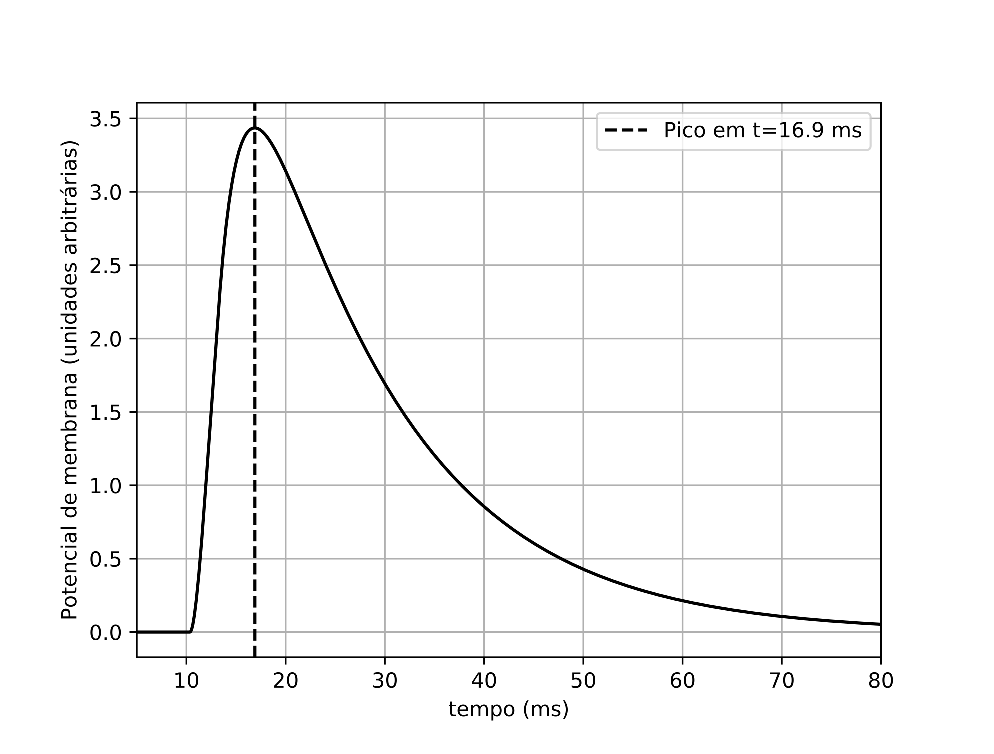
\includegraphics[scale=0.8]{EPSP.eps}
    \caption[PEPS em uma CR.]{Potencial excitat�rio p�s sin�ptico 
        em uma c�lula de Renshaw.}
	\label{fig:RCepsp}
\end{figure}

\subsubsection{Limita��es}
O tipo de estimula��o utilizado no experimento pode facilmente recrutar
mais de um MN. Dessa forma, a parametriza��o n�o levou em conta a
amplitude do PEPS. Esse caracter�stica, juntamente com a for�a sin�ptica
dessa conex�o, foi analisada junto com estudos
sobre conectividade e ser� abordado na se��o \ref{sec:conn}.

O tempo de subida foi um pouco maior do que o utilizado por
\citeonline{williams09}. O aumento da resist�ncia espec�fica aumentaria
o tempo de subida aqui apresentado, mas isso causaria um aumento
na dura��o do PEPS. Sendo assim, a parametriza��o realizada foi tomada
para satisfazer razoavelmente as duas caracter�sticas.

\subsection{Caracter�sticas dos disparos das C�lulas de Renshaw}
Quando o potencial de membrana do modelo da CR utilizado
ultrapassa o limiar de disparo, a condut�ncia de s�dio � acionada e
inicia a despolariza��o da c�lula. Por outro lado, as condut�ncias de 
pot�ssio r�pida e lenta causam a repolariza��o, sendo que esta
�ltima tem mais influ�ncia sob a p�s hiperpolariza��o (do ingl�s
\textit{afterhyperpolarization}, AHP) da c�lula.

A AHP � uma importante caracter�stica da CR. Antes de fazer essa
parametriza��o, entretanto, � preciso definir quando ela ir� disparar
um potencial de a��o. Sabe-se que essas c�lulas possuem
baixo limiar \cite{uchiyama03a}, mas n�o existem estudos quantitativos
especificamente sobre esse par�metro. O valor do limiar � calculado como

\begin{equation}
V_{l}=\frac{I_rR_m}{a}
\label{eq:vth}
\end{equation}

com $V_l$ sendo a tens�o de limiar, $I_r$ a corrente de reobase e $a$ a 
�rea superficial total. 

Outra caracter�stica afetada pela din�mica das condut�ncias dependentes
da voltagem � a curva de frequ�ncia de disparo \textit{versus} corrente
injetada (FxI), que tamb�m reflete a forma como a CR se adapta a uma
dada corrente.

Os par�metros de limiar, comprimento, di�metro e intensidade e din�mica
das condut�ncias do modelo da CR podem ser alterados para reproduzir as
caracter�sticas citadas. As parametriza��es feitas 
para obt�-los s�o baseadas nas seguintes refer�ncias:

\begin{itemize}
    \item \citeonline{hultborn79}: Curvas de FxI para diferentes correntes
        (Figura \ref{fig:HP79}\subref{fig:fxiRC}),
        sendo que os disparos s� come�am a ocorrer por volta de 0.5 nA.
        AHP ap�s um breve pulso de corrente injetada apresentou uma 
        amplitude de -2 mV e dura��o por volta de 30 ms
        (Figura \ref{fig:HP79}\subref{fig:AHPRC}).
    \item \citeonline{fyffe90}: Di�metro m�dio de 27 $\mu$m.
    \item \citeonline{bui03}: �rea superficial m�dia do soma e do dendrito
        de 1753.8 $\mu\text{m}^2$ e 16756 $\mu\text{m}^2$, respectivamente.
\end{itemize}

Usando o $R_m$ obtido na se��o anterior,
$a=\text{1753.8+16756 }\mu\text{m}^2$ e considerando que $I_r=\text{0.5 }$ nA,
a Equa��o (\ref{eq:vth}) resulta em $V_l=\text{22.9678 }$ mV.
Tomando a CR por um cilindro, sua �rea superficial total ser� 
$a=\text{1753.8+16756}=\pi ld$. Dessa forma, $l=\text{218.2168 }\mu$m.

Com esses valores, torna-se poss�vel parametrizar a AHP e a curva FxI.
Como o modelo de condut�ncia utilizado � baseado em pulsos \cite{destexhe94a},
as vari�veis de ativa��o de cada condut�ncia podem ser expressas como 
exponenciais com taxas de crescimento ou decaimento dependendo de vari�veis
de transi��o.

As vari�veis de transi��o $\alpha_N$ e $\beta_N$, relacionadas com a
din�mica dos canais de pot�ssio r�pido, foram aumentadas para que esses
canais se fechassem antes da membrana voltar ao n�vel de repouso (0 mV). 
Sendo assim, os canais de pot�ssio lento, com $\alpha_Q$ e $\beta_Q$,
puderam ser ajustados para se obter as taxas de disparos e adapta��o
apropriados.

O valor de $\beta_Q$ foi ajustado at� se obter uma localiza��o do pico da
AHP semelhante � da Figura \ref{fig:HP79}\subref{fig:AHPRC},
que se encontra mais ao centro de sua dura��o. Isso significa
alterar a velocidade de fechamento do canal para que este se n�o se feche
muito pr�ximo ao in�cio da AHP.

Considerando uma sequ�ncia de potenciais
de a��o, uma diminui��o no valor de $\alpha_Q$ faz com que o decaimento
da exponencial da vari�vel de ativa��o seja mais lento. Isso permite que 
estes possam se sobrepor, fazendo com que exista uma corrente i�nica
abaixando o potencial de membrana para o equil�brio do canal de pot�ssio
lento (-10 mV). Inicialmente, essa corrente � relativamente pequena, mas
ela cresce de forma cumulativa at� o momento em que os efeitos das primeiras
exponenciais gerando essa corrente desapare�a. Esse fen�meno, ent�o, gera 
uma adapta��o na frequ�ncia de disparo das CRs.

Por fim, a amplitude do AHP foi obtida ajustando os valores m�ximos
das condut�ncias de pot�ssio r�pida e lenta.

Detalhes sobre a AHP podem ser visto na Figura \ref{fig:RCahp}. O pico 
observado foi de -2 mV. Sua dura��o foi de aproximadamente 35 ms,
calculada de 15 ms at� o instante com 10\% do valor do pico, que foi em
50 ms.

\begin{figure}[ht!]
	\center
	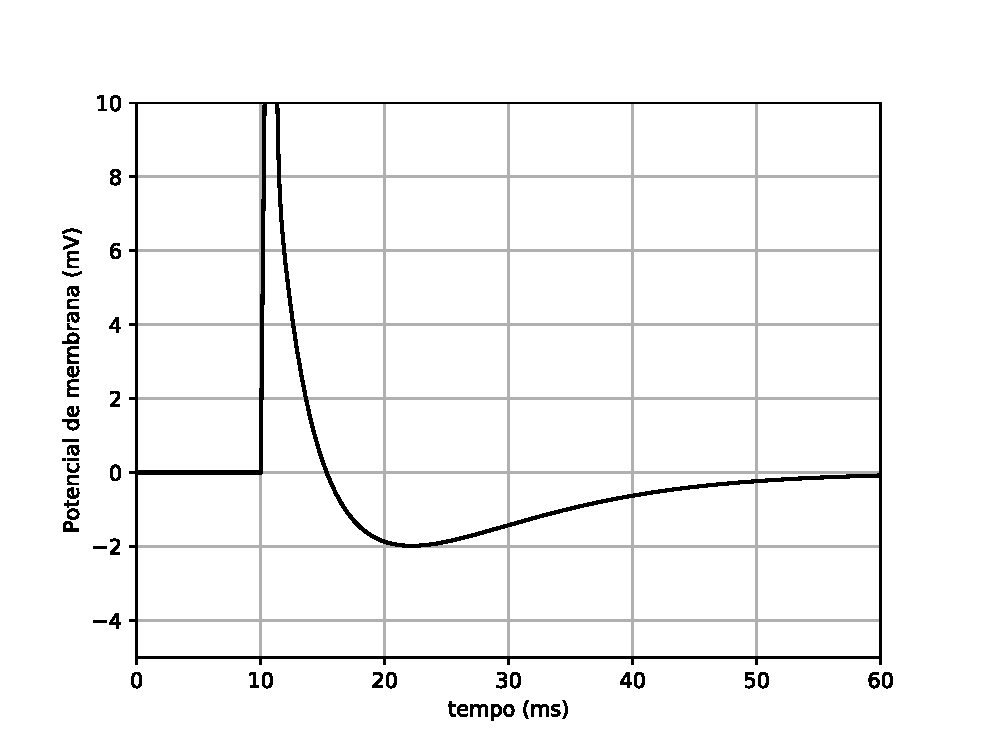
\includegraphics[scale=0.8]{AHP.eps}
    \caption[AHP em uma CR.]{P�s hiperpolariza��o de
        uma c�lula de Renshaw.}
	\label{fig:RCahp}
\end{figure}

A curva FxI obtida � mostrada na Figura \ref{fig:RCfxi}.
O primeiro e segundo potencial de a��o � entendido como o 
primeiro potencial, enquanto que o segundo e terceiro � o
segundo intervalo, e assim por diante. O regime estacion�rio foi
considerado como sendo ap�s 80 ms. A satura��o observada foi 
causada pela per�odo refrat�rio absoluto da c�lula, que � de 1 ms.

\begin{figure}[ht!]
	\center
	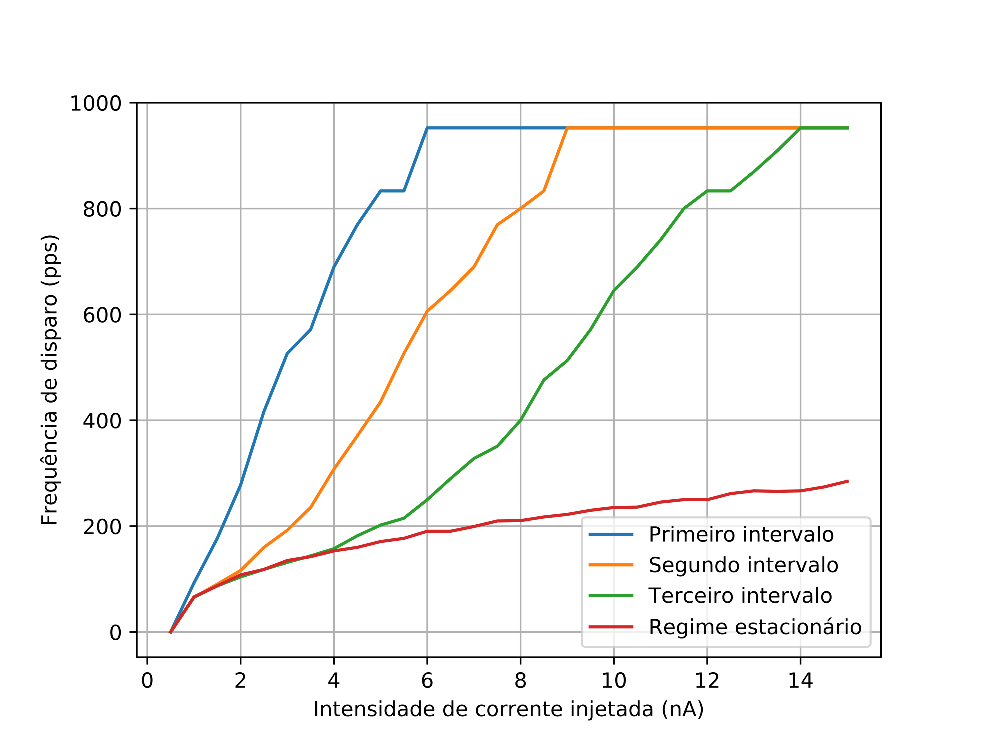
\includegraphics[scale=0.8]{FxI.eps}
    \caption[FxI em uma CR.]{Curva de frequ�ncia de disparo
    \textit{versus} corrente injetada de uma c�lula de Renshaw.}
	\label{fig:RCfxi}
\end{figure}

Com os resultados obtidos, a resist�ncia de entrada $R_i=\frac{R_m}{a}$
resultante foi de 45.92 M$\Omega$. Como esperado, esse valor � maior que 
a resist�ncia de entrada do menor MN.

\subsubsection{Limita��es}
A curva FxI apresentada se aproximou do que foi descrito na literatura, 
mas o tempo de dura��o da adapta��o, que � maior para correntes mais
altas, n�o. Em geral, essa dura��o foi sempre menor no modelo aqui descrito.
Isso � ilustrado na Figura \ref{fig:FxIcomp}.

\begin{figure}[ht]
    \centering
    \subfloat[][]{
        \label{fig:refmemb}
        \includegraphics[scale=0.8]{refmemb}
    }
    \hspace{-1cm}
    \subfloat[][]{
        \label{fig:resmemb}
        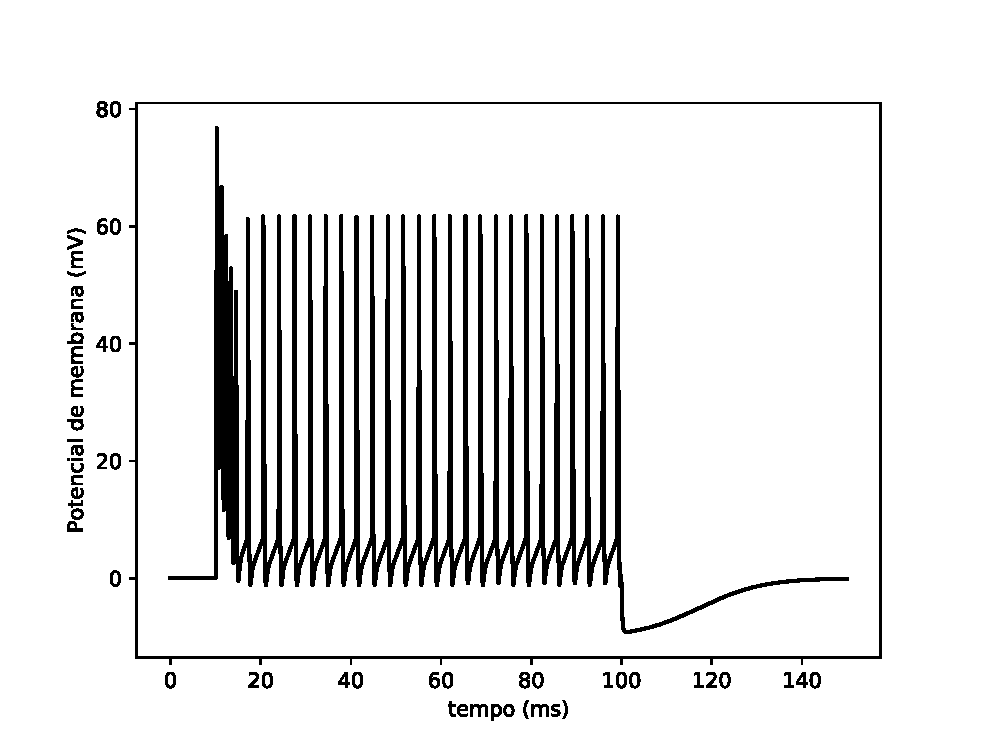
\includegraphics[scale=0.4]{FxI_RC.eps}
    }
    \caption[Compara��o dos potenciais de membrana para uma corrente injetada
        de 12 nA]{
        Compara��o dos potenciais de membrana para uma corrente injetada
        de 12 nA. \subref{fig:refmemb}  Tempo da adapta��o em uma
        CR tem uma dura��o de aproximadamente 30 ms \cite{hultborn79}.
        \subref{fig:resmemb} Resultado obtido pelo modelo de uma CR nas
        mesmas condi��es.
         }
    \label{fig:FxIcomp}
\end{figure}

\subsection{Potencial inibit�rio p�s sin�ptico de c�lula de Renshaw}
As condut�ncias das CRs sobre cada tipo de MN foram ajustadas, levando em
conta os seguintes dados experimentais:

\begin{itemize}
    \item \citeonline{vankeulen79}: PIPS em MNs causados por CRs.
    \item \citeonline{fyffe91}: Conex�es sin�pticas de CRs para MNs do 
        tipo $\alpha$ s�o localizadas nos dendritos.
    \item \citeonline{uchiyama03a}: Procedimento para estimar PIPS de
        acordo com o tipo de MN.
\end{itemize}

Ap�s sucessivas simula��es, o resultado final obtido � mostrado na 
Figura \ref{fig:PIPSres}. Os picos foram de -26.12 $\mu$V, -14.03 $\mu$V e
-7.00 $\mu$V para MNs do tipo S, FR e FF, respectivamente.

\begin{figure}[ht!]
	\center
	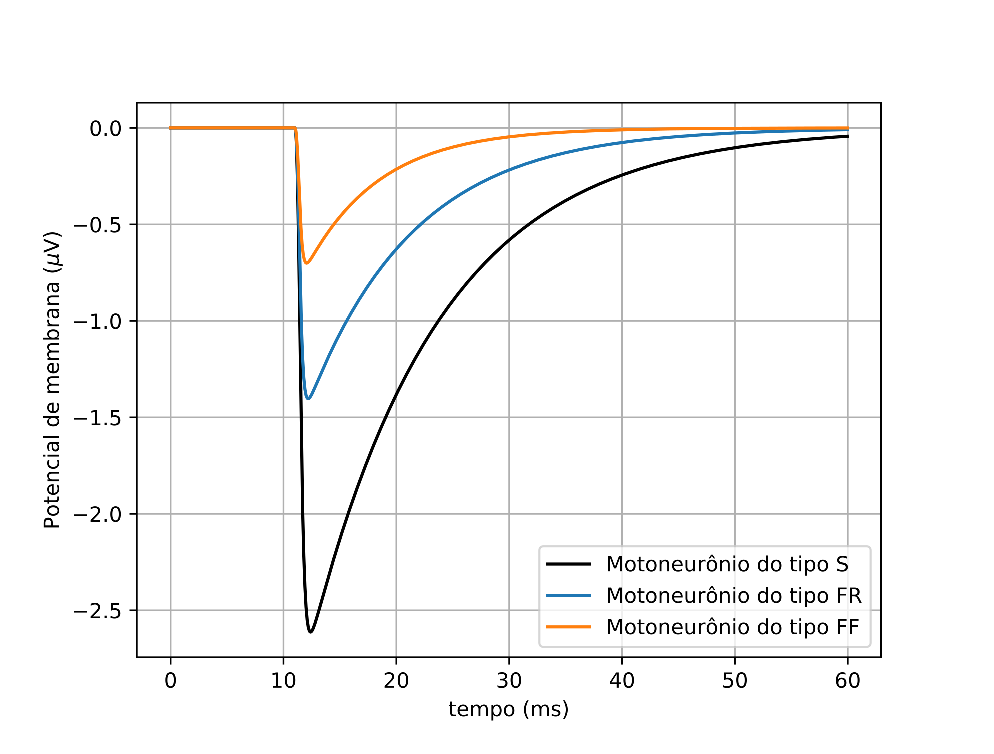
\includegraphics[scale=0.8]{IPSP.eps}
    \caption[PIPS de uma CR.]{Potencial inibit�rio p�s sin�ptico
        de c�lula de Renshaw em diferentes tipos de motoneur�nios.}
	\label{fig:PIPSres}
\end{figure}

\subsection{Atividade espont�nea da c�lula de Renshaw}
Para obter uma taxa de disparos espont�neos de 7 pps \cite{walmsley81},
foi necess�rio alterar o valor da condut�ncia m�xima do ru�do agindo sobre
a CR. Como visto na Figura \ref{fig:spont}, a taxa est� condizente com 
o esperado.

\begin{figure}[ht!]
	\center
	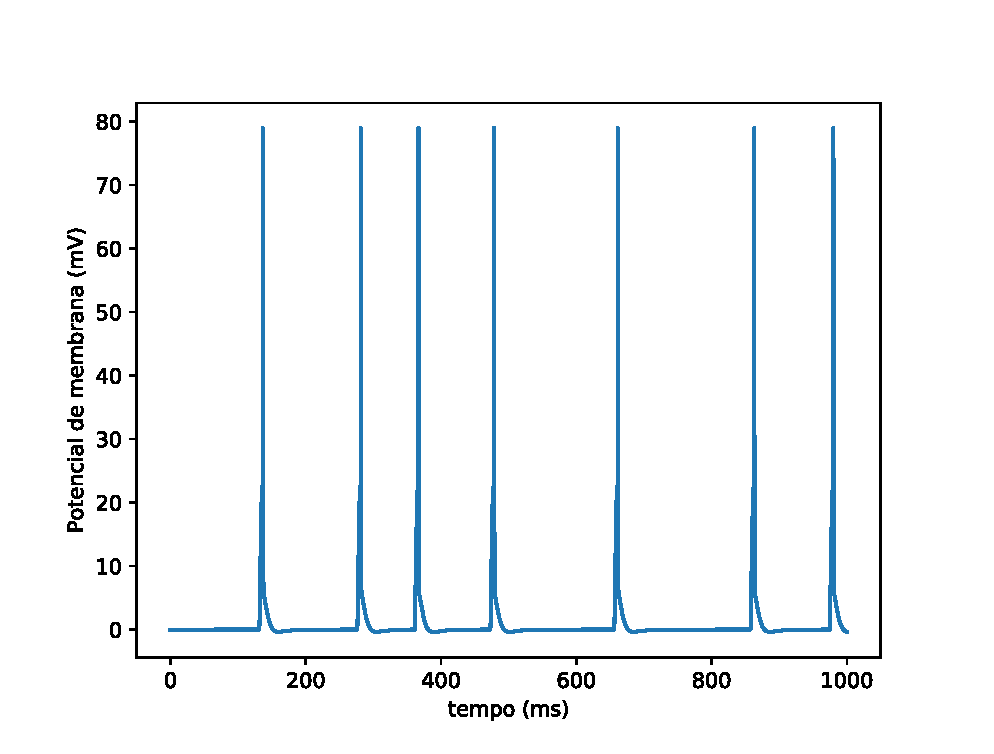
\includegraphics[scale=0.8]{spont.eps}
    \caption[Disparos espont�neos de uma CR.]{Disparos espont�neos de uma CR.}
	\label{fig:spont}
\end{figure}

\subsection{Conectividade do Circuito de Inibi��o Recorrente}
\label{sec:conn}
O grau de conectividade dos elementos que comp�em o circuito de
inibi��o recorrente envolve n�o s� a quantidade de elementos se
conectando, mas tamb�m a for�a de conex�o entre eles. Esses dois
par�metros ser�o ajustados baseados nas refer�ncias apresentadas
abaixo:

\begin{itemize}
    \item \citeonline{mccurdy94}: Distribui��o topogr�fica das amplitudes
        de PIPS recorrentes obtida de pares de MNs � inversamente
        correlacionada com a dist�ncia. Os autores fornecem uma vis�o
        geral, independente do n�cleo motor. MNs de m�sculo gastrocnemius
        medial separados por no m�ximo 1 mm s�o classificados como 
        pr�ximos. Fora dessa zona, s�o considerados distantes.
    \item \citeonline{hamm87b}: Distribui��o de amplitudes, tempo
        de meia vida e tempo de subida de PIPS recorrentes.
    \item \citeonline{uchiyama03a}: Padr�o de distribui��o topogr�fica 
        da for�a sin�ptica � o de uma gaussiana que decresce na medida
        em que se afasta do neur�nio pr� sin�ptico. O desvio padr�o da
        curva � de 0.167 mm e 1.164 mm para os MNs e para as CRs, 
        respectivamente. A quantidade de bot�es sin�pticos tamb�m �
        um indicativo da for�a sin�ptica das conex�es. Estima-se que os
        ax�nios colaterais dos MNs que alcan�am a regi�o onde as CRs se
        encontram possuam 78.5 $\pm$ 7.5, 43.0 $\pm$ 4.2 e 35.5 $\pm$ 3
        destas estruturas se forem do tipo FF, FR e S, respectivamente.
\end{itemize}

Para reproduzir o experimento como em \citeonline{mccurdy94}, as simula��es
consistiram em correntes injetadas no soma dos MNs por um curto per�odo de 
tempo. Foram levados em conta 180 pares, separados por dist�ncias entre
86 $\mu$m e 4.7 mm. Os MNs do n�cleo motor simulado inervam o m�sculo
gastrocn�mios medial e, por isso, a dist�ncia que define se estes est�o
pr�ximos ou distantes um do outro � de 1 mm \cite{mccurdy94}. 

O padr�o de decaimento adotado foi o da gaussiana da refer�ncia. O n�mero
de bot�es sin�pticos de cada tipo de MN nas CRs foi implementado como valores
de condut�ncia seguindo uma propor��o de 1:0.55:0.45 (FF:FR:S). Isso
permitiu que apenas a condut�ncia m�xima dos MNs do tipo FF
($g_{max_{FF}}$) fosse parametrizado, sendo as outras ajustadas
de acordo com a propor��o.

Vale notar
que, dentre os dados dispon�veis, apenas os significativos e provenientes
de gatos decapitados foram usados \cite{mccurdy94,hamm87b}.

Ap�s uma s�rie de simula��es, o valor de $g_{max_{FF}}$ que mostrou os
resultados mais apropriados de acordo com a literatura foi 33 nS.
O efeito da utiliza��o desse par�metro na distribui��o topogr�fica dos
PIPS recorrentes pode ser visto na Figura \ref{fig:mchammdecay}. O
padr�o de decaimento com dist�ncia foi semelhantes ao que foi apresentado
na refer�ncia \cite{mccurdy94} e a m�dia das respostas calculadas entre
pares distantes e pr�ximos foram de -23.60 $\mu$V e -68.83 $\mu$V,
respectivamente. Comparados com os -19,63 $\pm$ 2,42 $\mu$V e 
-41.36 $\pm$ 7.19 $\mu$V para pares distantes e pr�ximos \cite{mccurdy94},
respectivamente, � poss�vel ver que os valores m�dios para pares pr�ximos
na simula��o � maior do que na realidade.

\begin{figure}[ht!]
	\center
	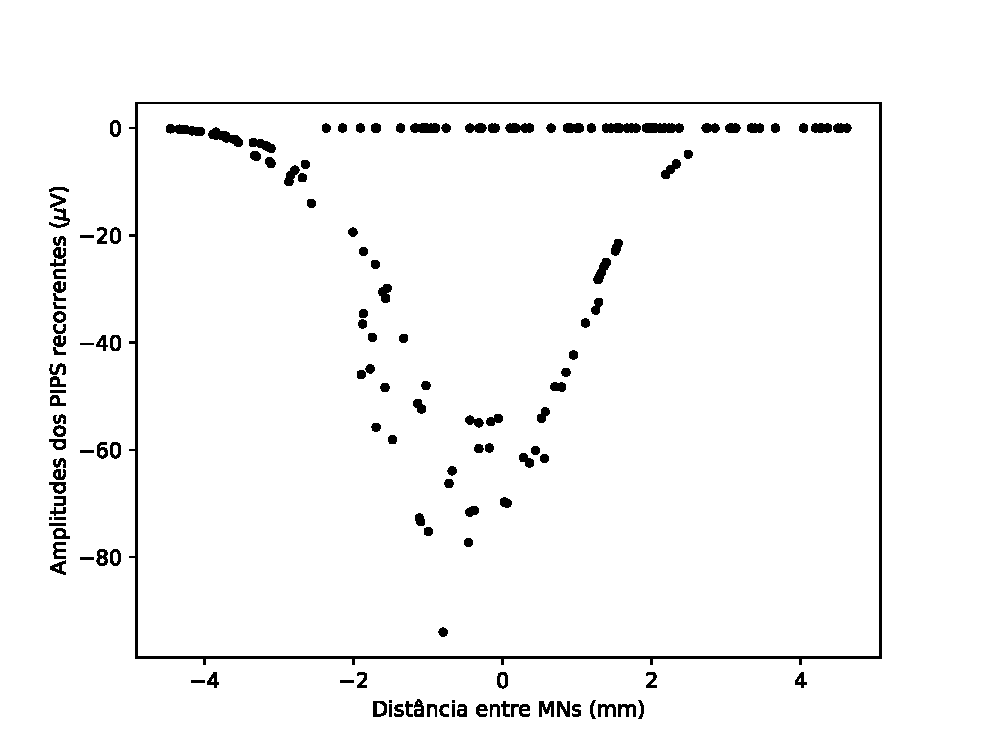
\includegraphics[scale=0.8]{mchammdecay.eps}
    \caption[Distribui��o topogr�fica de potenciais inibit�rios
            p�s sin�pticos recorrentes.]{Distribui��o topogr�fica de
            potenciais inibit�rios p�s sin�pticos recorrentes. Cada
            ponto representa a amplitude desses potenciais ap�s o est�mulo
            de outro motoneur�nio, localizado em zero na abcissa.
            Se observado em um motoneur�nio
            rostral (caudal) ao motoneur�nio estimulado, � apresentado
            na parte negativa (positiva) da abcissa.}
	\label{fig:mchammdecay}
\end{figure}

Um aumento ou diminui��o no valor de $g_{max_{FF}}$ mudaria o resultado
da m�dia dos PIPS recorrentes, mas isso tamb�m alteraria as distribui��es
de amplitudes dos PIPS, que, como mostrado na Figura
\ref{fig:mchammamplitude}, se mostrou dentro das faixas de valores
descritos na literatura. Pode-se perceber, entretanto,
que a forma como as alturas dos histogramas se distribuem foi diferente
do esperado \cite{hamm87b}. Vale notar que, com a condut�ncia
adotada, apenas MNs do tipo FF, ou seja, aqueles com �ndice maior do
que 149, s�o capazes de causar potenciais de a��o nas CRs e, assim, gerar
PIPS recorrentes.

\begin{figure}[ht!]
	\center
	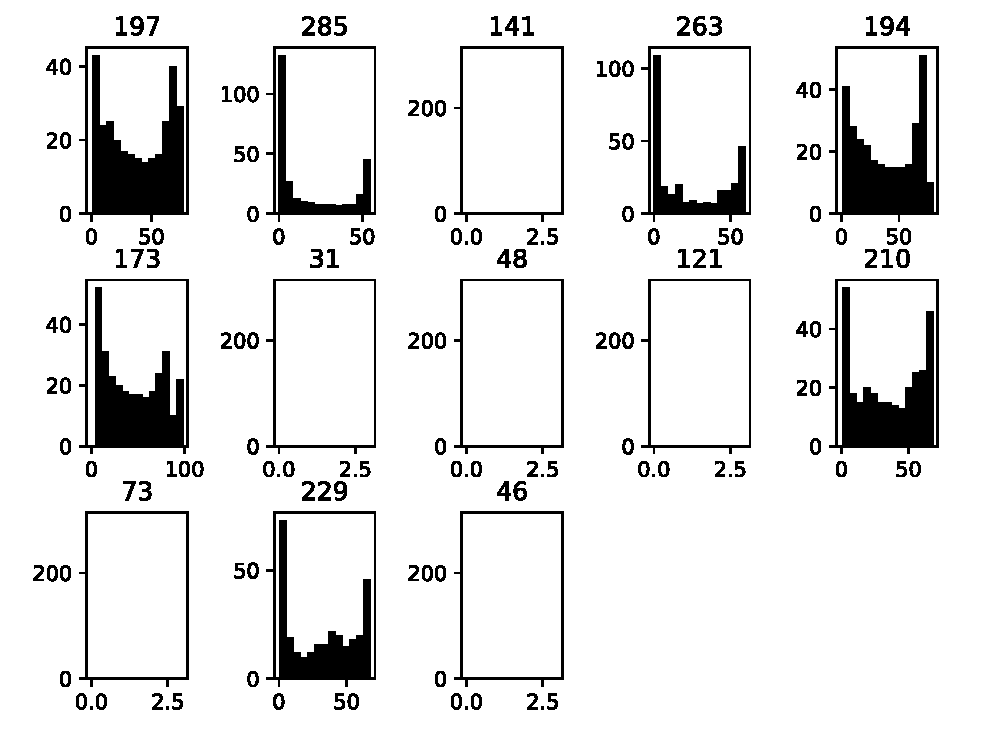
\includegraphics[scale=0.8]{mchammamplitude.eps}
    \caption[Distribui��o de amplitudes de potenciais inibit�rios
            p�s sin�pticos recorrentes.]{Distribui��o de amplitudes
            de potenciais inibit�rios p�s sin�pticos recorrentes. Em
            cada gr�fico, o n�mero na parte superior significa o
            �ndice do motoneur�nio estimulado. Eixo das abcissas 
            indica valores de amplitudes, em $\mu$V, e eixo das ordenadas
            indica quantidade. Gr�ficos vazios indicam a aus�ncia de 
            potenciais inibit�rios p�s sin�pticos recorrentes gerados
            pelo est�mulo de determinado motoneur�nio.}
	\label{fig:mchammamplitude}
\end{figure}

\subsubsection{Limita��es}
A compara��o por inspe��o visual dos resultados da Figura
\ref{fig:mchammdecay} com os de \citeonline{mccurdy94} mostra
consist�ncia no decaimento da for�a sin�ptica com a dist�ncia. 
Sabe-se que a amplitude de PIPS recorrentes entre pares de MNs pr�ximos
� relativamente vari�vel, sendo observados valores de -40 $\mu$V e
-280 $\mu$V para uma mesma dist�ncia, por exemplo. Os mecanismos
respons�veis por essa
caracter�stica, entretanto, s�o especulativos \cite{mccurdy94}.
Nos resultados aqui obtidos, esta variabilidade n�o foi observada
e, por isso, a m�dia de PIPS recorrentes
para pares de MNs pr�ximos foi maior do que o esperado.

Os histogramas de amplitude da Figura
\ref{fig:mchammamplitude} est�o dentro das faixas descritas na 
literatura \cite{hamm87b}. Existem registros de PIPS recorrentes 
maiores \cite{mccurdy94}, mas estes se manifestaram esporadicamente
e apenas para pares de MNs pr�ximos. O fato de alguns MNs n�o serem capazes 
de gerar PIPS recorrentes n�o � inapropriado pois existem estudos
mostrando que a ativa��o de CRs pode resultar em respostas como
aus�ncia, alguns e at� \textit{bursts} de potenciais de a��o
\cite{ross72,ross82}.

Vale notar que outros valores maiores de $g_{max_{FF}}$ geraram resultados
semelhantes, mas com amplitudes m�ximas e valores m�dios elevados e
baixa variabilidade, al�m de afetar negativamente os resultados de an�lise
est�tica da CR. Menores $g_{max_{FF}}$,
por sua vez, faria com que o efeito 
das CRs fosse muito baixo. Sendo assim, o valor de condut�ncia adotado
fornece um equil�brio razo�vel dos resultados.

Os par�metros apresentados nessa se��o, assim como seus valores, s�o
sumarizados na Tabela \ref{tab:params_final}.

\begin{table}[ht!]
\caption{Principais par�metros das c�lulas de Renshaw e seus valores.}
\label{tab:params_final}
\centering
    \begin{tabular}{c C{3cm} C{3cm}}\hline 
	Par�metro & Valor & Unidade \\ \hline 
    Resist�ncia espec�fica de membrana & 8500  & $\Omega\text{cm}^2$ \\
    Capacit�ncia espec�fica de membrana & 1  & $\mu\text{Fcm}^{-2}$ \\
    Corrente de reobase & 0.5 & nA \\
    Di�metro & 27 & $\mu$m \\
    Comprimento & 218.2168 & $\mu$m \\
    Limiar & 22.9608 & mV  \\ 
    $\alpha_N$ & 6 & ms$^{-1}$  \\ 
    $\beta_N$ & 0.5 & ms$^{-1}$ \\ 
    $\alpha_Q$ & 0.004 & ms$^{-1}$  \\ 
    $\beta_Q$ & 0.02 & ms$^{-1}$  \\ 
    Condut�ncia m�xima do canal de pot�ssio lento & 2300 & mS/cm$^2$ \\
    Condut�ncia m�xima do canal de pot�ssio r�pido & 3.3 & mS/cm$^2$ \\
    Condut�ncia m�xima CR - MN S & 128 & nS \\
    Condut�ncia m�xima CR - MN FR & 119 & nS \\
    Condut�ncia m�xima CR - MN FF & 94 & nS \\
    Condut�ncia m�xima do ru�do & 30.15 & nS \\
    Condut�ncia m�xima MN S - CR & 15 & nS \\
    Condut�ncia m�xima MN FR - CR & 18.33 & nS \\
    Condut�ncia m�xima MN FF - CR & 32 & nS \\
	\hline
    \end{tabular}
\end{table}


	\section{Valida��es}
\label{sec:val}
Nesta se��o, a robustez da parametriza��o adotada foi testada por meio
da compara��o de resultados de procedimentos experimentais com resultados
obtidos de simula��es desses experimentos.

\subsection{Caracter�sticas de potenciais inibit�rios
            p�s sin�pticos recorrentes}
Os resultados de simula��o para o tempo de subida e tempo de meia vida s�o
mostrados na Figura \ref{fig:mchammvalidation} abaixo. Como pode ser visto,
esses tiveram faixas consideravelmente abaixo dos valores
esperados \cite{hamm87b}. Apesar disso, algumas semelhan�as existem: ambos
s�o distorcidos � direita e o histograma do tempo de subida � bimodal.

\begin{figure}[ht]
    \centering
    \subfloat[][]{
        \label{fig:mchammrise}
        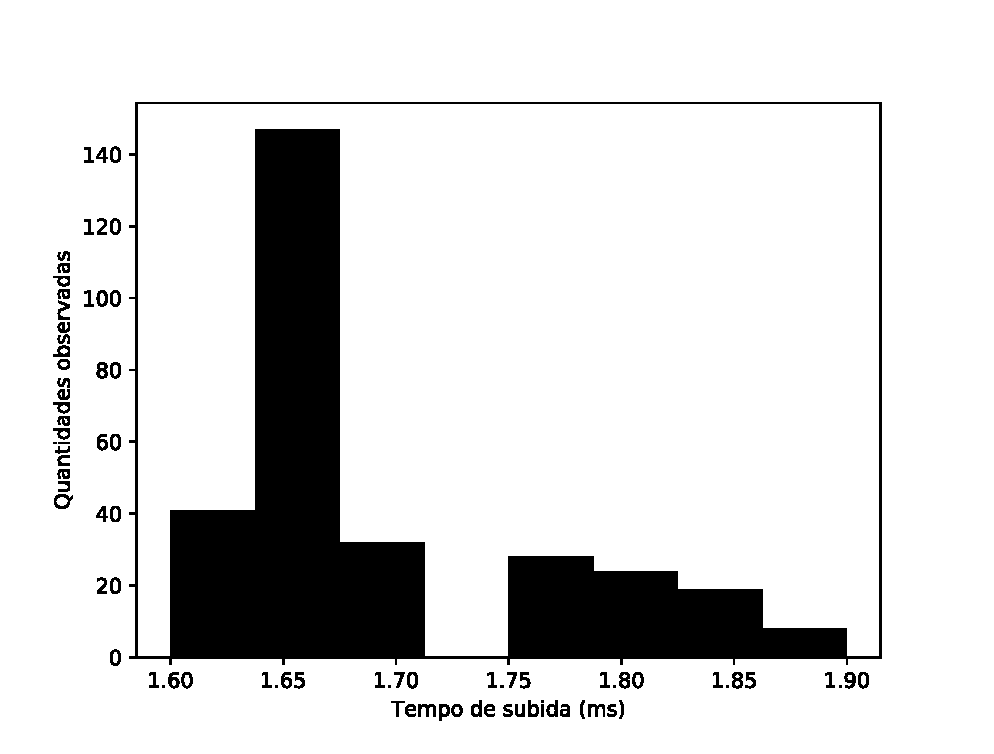
\includegraphics[scale=0.5]{mchammrise.eps}
    }
    \hspace{-1cm}
    \subfloat[][]{
        \label{fig:mchammwidth}
        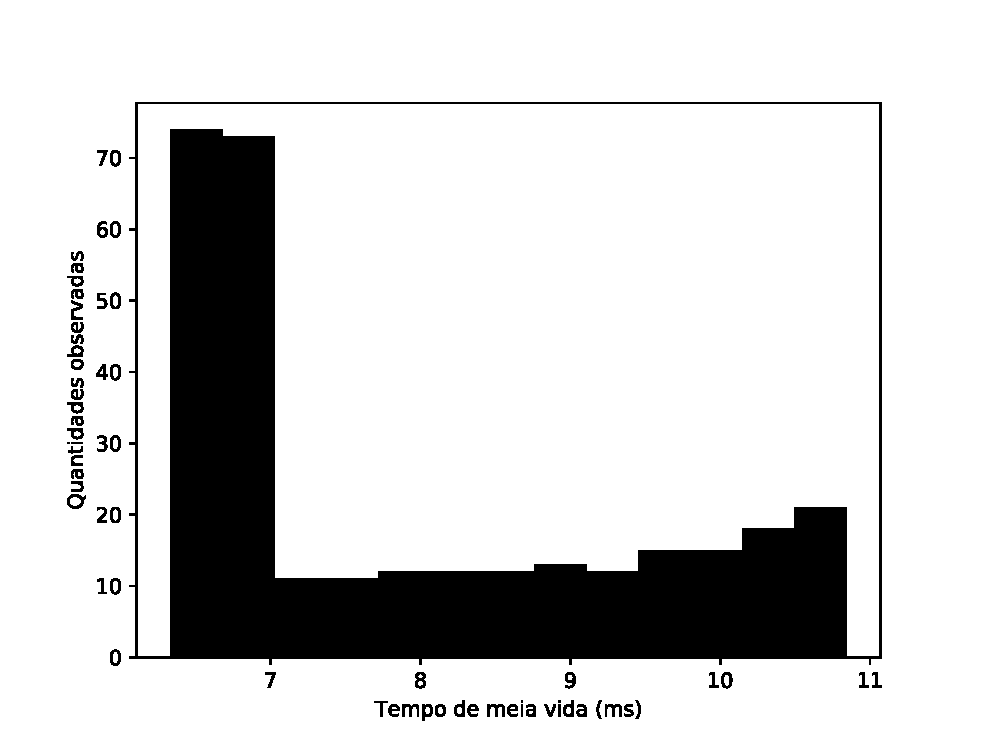
\includegraphics[scale=0.5]{mchammwidth.eps}
    }
    \caption[Valida��o de resultados com \citeonline{hamm87b}.]{
        Valida��o de resultados com \citeonline{hamm87b}.
        \subref{fig:mchammrise} Tempo de subida dos potenciais inibit�rios
        p�s sin�pticos gravados.
        \subref{fig:mchammwidth} Tempo de meia vidas dos potenciais
        inibit�rios p�s sin�pticos gravados.
         }
    \label{fig:mchammvalidation}
\end{figure}

Pode-se perceber, entretanto,
que a forma como as alturas dos histogramas se distribuem foi diferente
do esperado \cite{hamm87b}. Vale notar que, com a condut�ncia
adotada, apenas MNs do tipo FF, ou seja, aqueles com �ndice maior do
que 149, s�o capazes de causar potenciais de a��o nas CRs e, assim, gerar
PIPS recorrentes.

\begin{figure}[ht!]
	\center
	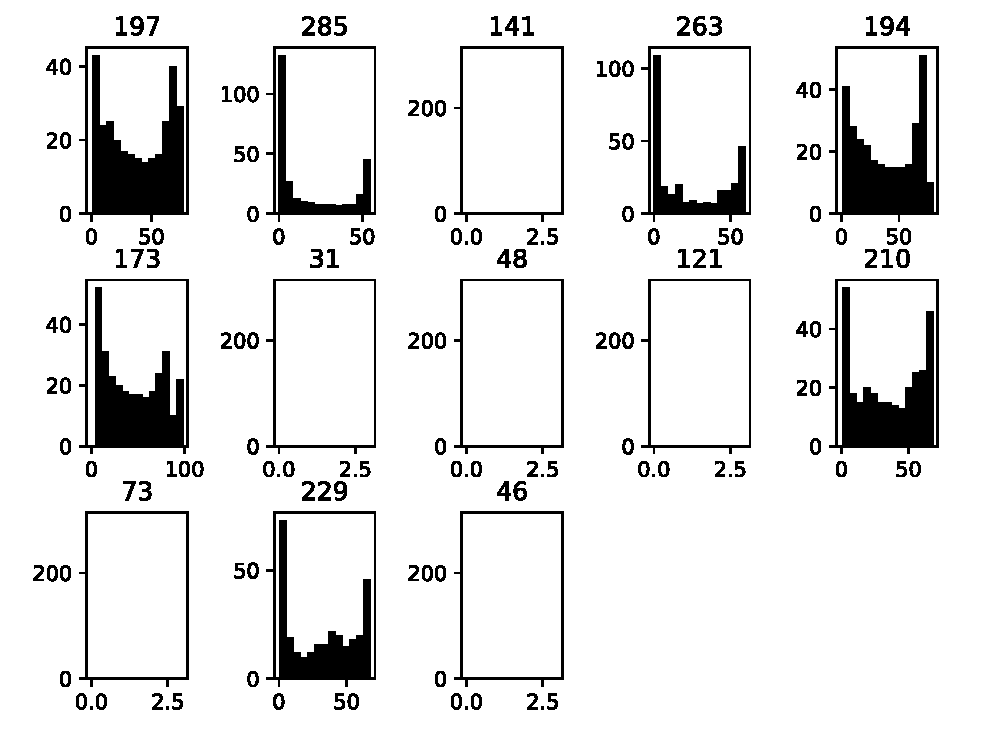
\includegraphics[scale=0.8]{mchammamplitude.eps}
    \caption[Distribui��o de amplitudes de potenciais inibit�rios
            p�s sin�pticos recorrentes.]{Distribui��o de amplitudes
            de potenciais inibit�rios p�s sin�pticos recorrentes. Em
            cada gr�fico, o n�mero na parte superior significa o
            �ndice do motoneur�nio estimulado. Eixo das abcissas 
            indica valores de amplitudes, em $\mu$V, e eixo das ordenadas
            indica quantidade. Gr�ficos vazios indicam a aus�ncia de 
            potenciais inibit�rios p�s sin�pticos recorrentes gerados
            pelo est�mulo de determinado motoneur�nio.}
	\label{fig:mchammamplitude}
\end{figure}

Os histogramas de amplitude da Figura
\ref{fig:mchammamplitude} est�o dentro das faixas descritas na 
literatura \cite{hamm87b}. Existem registros de PIPS recorrentes 
maiores \cite{mccurdy94}, mas estes se manifestaram esporadicamente
e apenas para pares de MNs pr�ximos. O fato de alguns MNs n�o serem capazes 
de gerar PIPS recorrentes n�o � inapropriado pois existem estudos
mostrando que a ativa��o de CRs pode resultar em respostas como
aus�ncia, alguns poucos e at� \textit{bursts} de potenciais de a��o
\cite{ross72,ross82}.

\subsection{Rela��o est�tica das entradas e sa�das das c�lulas de renshaw}
A rela��o est�tica de entrada e sa�da realizada por \citeonline{cleveland81}
� importante para a caracteriza��o de CRs. Foi observado que os resultados
obtidos poderiam ser ajustados a uma fun��o hiperb�lica, que por
conveni�ncia foi chamada de fun��o de Langmuir pelos autores. Esta abordagem
tamb�m foi empregada nesse trabalho e a fun��o em quest�o foi calculada como

\begin{equation}
    f_{CR}=\frac{cf_{AD}}{k+f_{AD}}
\end{equation}

em que $f_{AD}$ � a frequ�ncia do est�mulo, $f_{CR}$ � a taxa de disparo
m�dia da CR ap�s adapta��o, $c$ � a constante de satura��o e $k$ � a 
constante de semi satura��o. Esta an�lise foi reproduzida
no modelo parametrizado, passado um per�odo de adapta��o do neur�nio e 
considerando as frequ�ncias de est�mulos antidr�micos como entrada e
taxas de disparos das CRs como sa�da.

Os resultados s�o apresentados na Figura \ref{fig:static}. A Figura 
\ref{fig:static24} mostra que as curvas obtidas de 24 CRs diferentes
n�o apresentaram uma satura��o t�o clara quanto as das descritas na
literatura, de forma que, para taxas menores de est�mulos antidr�micos,
as taxas de disparos das CRs n�o aumentaram t�o r�pido quanto deveriam.
Apesar disso, suas taxas de disparos m�ximas estiveram dentro das faixas de
valores esperados, que v�o de aproximadamente 50 at� 290 pps. A Figura 
\ref{fig:staticnorm} corrobora com esses resultados e mostra que a m�dia
das curvas foi um pouco menor do que o esperado.

\begin{figure}[ht]
    \centering
    \subfloat[][]{
        \label{fig:static24}
        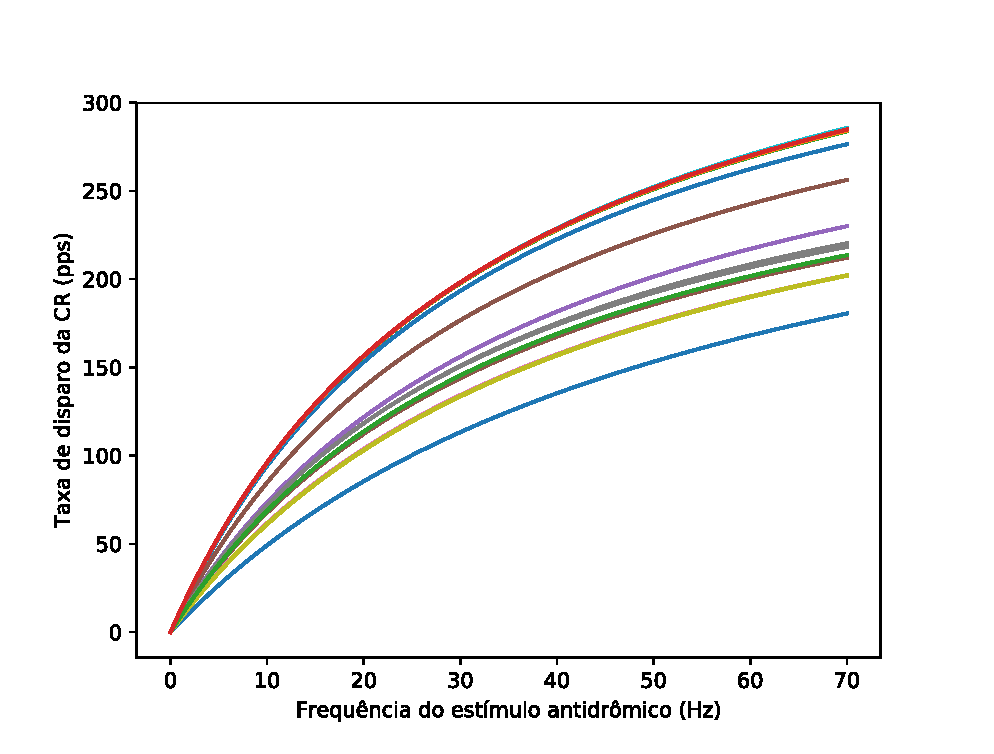
\includegraphics[scale=0.5]{static24.eps}
    }
    \hspace{-1cm}
    \subfloat[][]{
        \label{fig:staticnorm}
        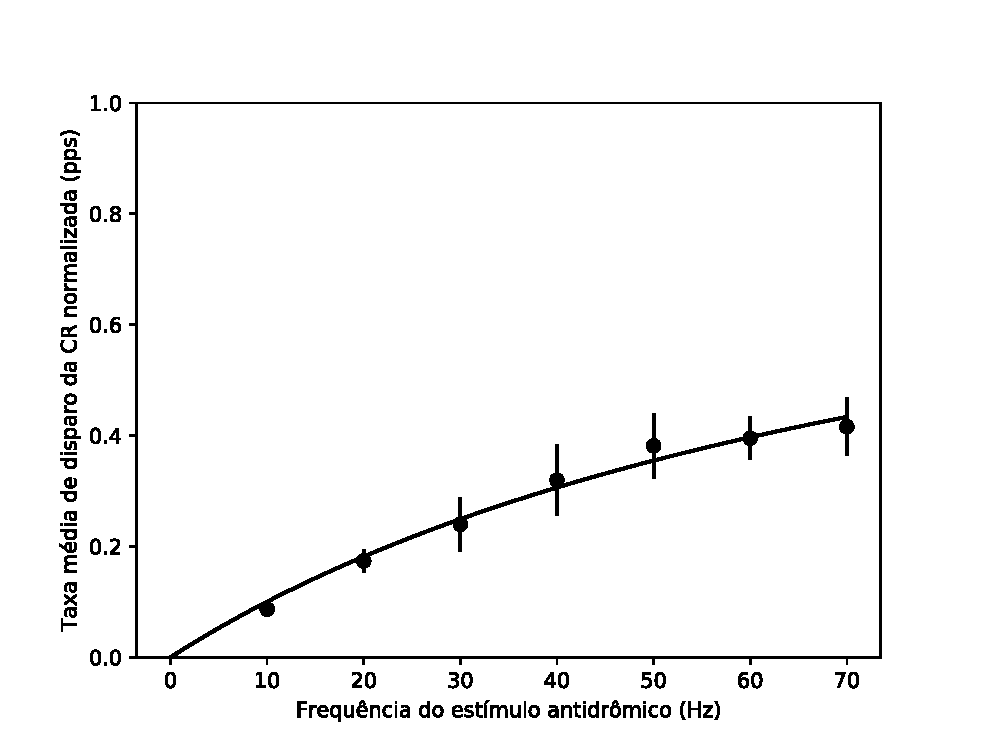
\includegraphics[scale=0.5]{staticnorm.eps}
    }
    \caption[Rela��es de entrada e sa�da de CRs.]{
        Rela��es de entrada e sa�da de c�lulas de Renshaw.
        \subref{fig:static24} Ajustes de fun��es de Langmuir � respostas
        de 24 c�lulas de Renshaw escolhidas ao acaso 
        (representadas cada uma por diferentes
        cores) sujeitas a diferentes taxasupram�ximade est�mulo.
        \subref{fig:staticnorm} M�dia normalizada das curvas obtidas
        ajustada � uma fun��o de Langmuir. Os pontos s�o as m�dias e 
        as barras verticais s�o os desvios padr�es.
         }
    \label{fig:static}
\end{figure}

Vale notar 
que o efeito de um est�mulo antidr�mico em CRs pr�ximas uma das outras
� muito parecido e em alguns casos, como visto na Figura \ref{fig:static24},
estas aparecem sobrepostas. Isso � consistente com o fato de que a taxa de 
disparo de uma CR est� relacionada com dois tipos de entrada: a sua taxa de
ativa��o e o n�mero de sinapses excitat�rias agindo sobre ela
\cite{cleveland81}, sendo este �ltimo, no modelo estudado neste
trabalho, entendido como condut�ncias sin�pticas. Dessa forma, � de 
se esperar que em regi�es com popula��es localmente homog�neas
de MNs as CRs ali presentes recebam uma entrada parecida.

\subsection{Respostas das c�lulas de renshaw sujeitas � um est�mulo
            antidr�mico}
Outro resultado bem conhecido das CRs � o de que estas, quando estimuladas
por um �nico pulso capaz de ativar todos os ax�nios motores fornecendo
inibi��o recorrente para as mesmas, exibem disparos que
podem durar at� algumas dezenas de milissegundos e taxas de disparos
instant�neas decrescentes com o tempo e dependentes da for�a sin�ptica 
total \cite{eccles61b,uchiyama03a}.

Como mostrado na Figura \ref{fig:firing}, o modelo parametrizado foi
capaz de reproduzir essas caracter�sticas. Houveram salvas de potenciais
de a��o com dura��o de 40 ms e suas taxas de disparo deca�ram de forma 
semelhante � uma exponencial. Com o est�mulo de 67.2 \%, que �
suficiente para ativar apenas os ax�nios motores dos MNs do tipo FF,
o n�mero de disparos e a dura��o da salva foram menores, pois 
existe uma for�a sin�ptica total menor agindo sobre a CR.

\begin{figure}[ht!]
	\center
	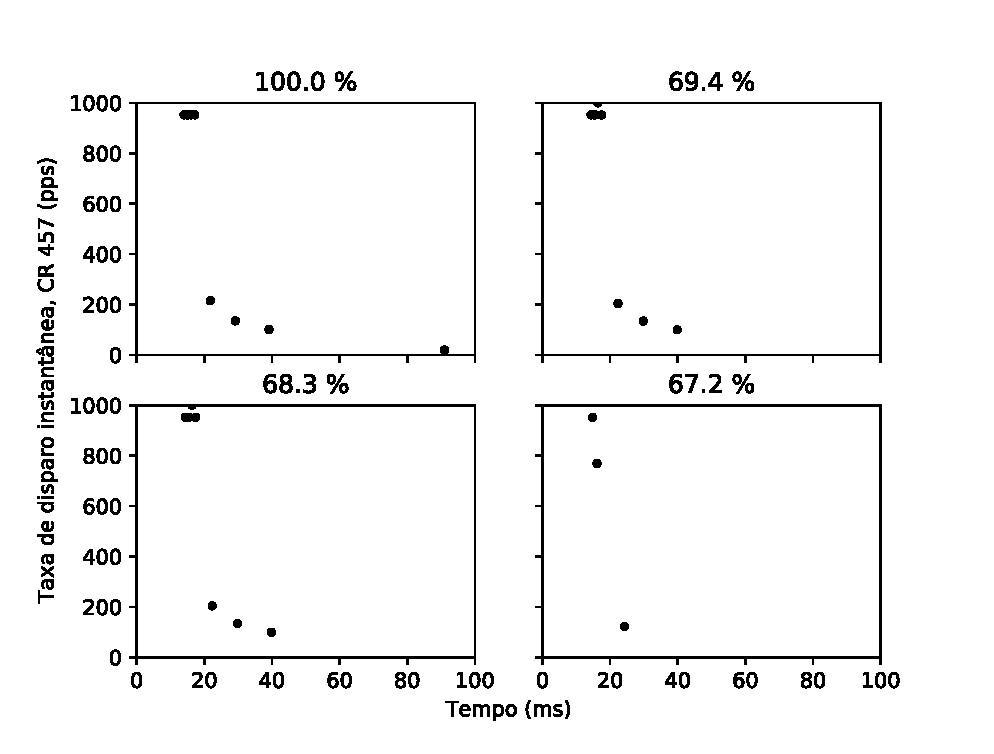
\includegraphics[scale=0.8]{firing.eps}
    \caption[Taxa de disparos intant�neos de uma CR ap�s um est�mulo
             antidr�mico.]{Taxa de disparos instant�neos da CRs de �ndice
             457 ap�s um est�mulo antidr�mico. As porcentagens indicam
             a intensidade do est�mulo, sendo 100 \% o caso em que
             todos os ax�nios motores s�o ativados.
             }
	\label{fig:firing}
\end{figure}

O tipo de est�mulo utilizado ativa muitos
ax�nios motores sincronizadamente, criando uma resposta artificial que 
raramente ocorre naturalmente \cite{uchiyama03a}. Apesar disso, esse
resultado � �til para validar a parametriza��o das CRs.

Vale notar que a taxa m�xima de disparos n�o ultrapassou 1000 pps, conforme
mostram \citeonline{hultborn79}. Isso � causado pela defini��o de
1 ms como per�odo refrat�rio absoluto das CRs.

	\section{estudos de hip�teses com o ReMoto}

\subsection{controle da for�a}

	\chapter{Conclus�es}
Os resultados relativos ao desempenho computacional apontam poss�veis
melhorias para o ReMoto.
A implementa��o de uma matriz de condut�ncias adequada para opera��es
vetorizadas foi, inclusive, incorporada na vers�o do ReMoto em 
Fortran. A utiliza��o de \textit{clusters}, por sua vez, seria mais
complexa e envolveria modifica��es consider�veis no c�digo.

A parametriza��o dos MNs e CRs foi realizada baseando-se em dados
experimentais e os resultados foram satisfat�rios. Caracter�sticas
din�micas e de depress�o p�s-sin�pticas n�o puderam ser
reproduzidas, mas essas limita��es foram discutidas e consideradas dentro
do contexto apropriado.

	
	\ProximoForaDoSumario
	\bibliography{library}
	\setboolean{ABNTNextOutOfTOC}{false}
	
	%\apendice
	
	%\chapter{Ap�ndice}

\index{ap�ndice}
Este cap�tulo � um Ap�ndice da Tese. Ap�ndices s�o cap�tulos com conte�do criado pelo autor, mas que n�o faz parte do tema central da Tese/Disserta��o.
	
	
	%\anexo	
	%\chapter{Anexo}


\index{anexo}
Este cap�tulo � um Anexo da Tese. Anexos s�o cap�tulos com conte�do que n�o foi criado pelo autor da Tese/Disserta��o.
	\setboolean{ABNTNextOutOfTOC}{false}
  
  %\printindex
	
	
\end{document}

